\documentclass[]{book}
\usepackage{lmodern}
\usepackage{amssymb,amsmath}
\usepackage{ifxetex,ifluatex}
\usepackage{fixltx2e} % provides \textsubscript
\ifnum 0\ifxetex 1\fi\ifluatex 1\fi=0 % if pdftex
  \usepackage[T1]{fontenc}
  \usepackage[utf8]{inputenc}
\else % if luatex or xelatex
  \ifxetex
    \usepackage{mathspec}
  \else
    \usepackage{fontspec}
  \fi
  \defaultfontfeatures{Ligatures=TeX,Scale=MatchLowercase}
\fi
% use upquote if available, for straight quotes in verbatim environments
\IfFileExists{upquote.sty}{\usepackage{upquote}}{}
% use microtype if available
\IfFileExists{microtype.sty}{%
\usepackage{microtype}
\UseMicrotypeSet[protrusion]{basicmath} % disable protrusion for tt fonts
}{}
\usepackage[margin=1in]{geometry}
\usepackage{hyperref}
\hypersetup{unicode=true,
            pdftitle={Intermediate Statistics with R},
            pdfauthor={Mark C Greenwood},
            pdfborder={0 0 0},
            breaklinks=true}
\urlstyle{same}  % don't use monospace font for urls
\usepackage{natbib}
\bibliographystyle{plainnat}
\usepackage{color}
\usepackage{fancyvrb}
\newcommand{\VerbBar}{|}
\newcommand{\VERB}{\Verb[commandchars=\\\{\}]}
\DefineVerbatimEnvironment{Highlighting}{Verbatim}{commandchars=\\\{\}}
% Add ',fontsize=\small' for more characters per line
\usepackage{framed}
\definecolor{shadecolor}{RGB}{248,248,248}
\newenvironment{Shaded}{\begin{snugshade}}{\end{snugshade}}
\newcommand{\AlertTok}[1]{\textcolor[rgb]{0.94,0.16,0.16}{#1}}
\newcommand{\AnnotationTok}[1]{\textcolor[rgb]{0.56,0.35,0.01}{\textbf{\textit{#1}}}}
\newcommand{\AttributeTok}[1]{\textcolor[rgb]{0.77,0.63,0.00}{#1}}
\newcommand{\BaseNTok}[1]{\textcolor[rgb]{0.00,0.00,0.81}{#1}}
\newcommand{\BuiltInTok}[1]{#1}
\newcommand{\CharTok}[1]{\textcolor[rgb]{0.31,0.60,0.02}{#1}}
\newcommand{\CommentTok}[1]{\textcolor[rgb]{0.56,0.35,0.01}{\textit{#1}}}
\newcommand{\CommentVarTok}[1]{\textcolor[rgb]{0.56,0.35,0.01}{\textbf{\textit{#1}}}}
\newcommand{\ConstantTok}[1]{\textcolor[rgb]{0.00,0.00,0.00}{#1}}
\newcommand{\ControlFlowTok}[1]{\textcolor[rgb]{0.13,0.29,0.53}{\textbf{#1}}}
\newcommand{\DataTypeTok}[1]{\textcolor[rgb]{0.13,0.29,0.53}{#1}}
\newcommand{\DecValTok}[1]{\textcolor[rgb]{0.00,0.00,0.81}{#1}}
\newcommand{\DocumentationTok}[1]{\textcolor[rgb]{0.56,0.35,0.01}{\textbf{\textit{#1}}}}
\newcommand{\ErrorTok}[1]{\textcolor[rgb]{0.64,0.00,0.00}{\textbf{#1}}}
\newcommand{\ExtensionTok}[1]{#1}
\newcommand{\FloatTok}[1]{\textcolor[rgb]{0.00,0.00,0.81}{#1}}
\newcommand{\FunctionTok}[1]{\textcolor[rgb]{0.00,0.00,0.00}{#1}}
\newcommand{\ImportTok}[1]{#1}
\newcommand{\InformationTok}[1]{\textcolor[rgb]{0.56,0.35,0.01}{\textbf{\textit{#1}}}}
\newcommand{\KeywordTok}[1]{\textcolor[rgb]{0.13,0.29,0.53}{\textbf{#1}}}
\newcommand{\NormalTok}[1]{#1}
\newcommand{\OperatorTok}[1]{\textcolor[rgb]{0.81,0.36,0.00}{\textbf{#1}}}
\newcommand{\OtherTok}[1]{\textcolor[rgb]{0.56,0.35,0.01}{#1}}
\newcommand{\PreprocessorTok}[1]{\textcolor[rgb]{0.56,0.35,0.01}{\textit{#1}}}
\newcommand{\RegionMarkerTok}[1]{#1}
\newcommand{\SpecialCharTok}[1]{\textcolor[rgb]{0.00,0.00,0.00}{#1}}
\newcommand{\SpecialStringTok}[1]{\textcolor[rgb]{0.31,0.60,0.02}{#1}}
\newcommand{\StringTok}[1]{\textcolor[rgb]{0.31,0.60,0.02}{#1}}
\newcommand{\VariableTok}[1]{\textcolor[rgb]{0.00,0.00,0.00}{#1}}
\newcommand{\VerbatimStringTok}[1]{\textcolor[rgb]{0.31,0.60,0.02}{#1}}
\newcommand{\WarningTok}[1]{\textcolor[rgb]{0.56,0.35,0.01}{\textbf{\textit{#1}}}}
\usepackage{longtable,booktabs}
\usepackage{graphicx,grffile}
\makeatletter
\def\maxwidth{\ifdim\Gin@nat@width>\linewidth\linewidth\else\Gin@nat@width\fi}
\def\maxheight{\ifdim\Gin@nat@height>\textheight\textheight\else\Gin@nat@height\fi}
\makeatother
% Scale images if necessary, so that they will not overflow the page
% margins by default, and it is still possible to overwrite the defaults
% using explicit options in \includegraphics[width, height, ...]{}
\setkeys{Gin}{width=\maxwidth,height=\maxheight,keepaspectratio}
\IfFileExists{parskip.sty}{%
\usepackage{parskip}
}{% else
\setlength{\parindent}{0pt}
\setlength{\parskip}{6pt plus 2pt minus 1pt}
}
\setlength{\emergencystretch}{3em}  % prevent overfull lines
\providecommand{\tightlist}{%
  \setlength{\itemsep}{0pt}\setlength{\parskip}{0pt}}
\setcounter{secnumdepth}{5}
% Redefines (sub)paragraphs to behave more like sections
\ifx\paragraph\undefined\else
\let\oldparagraph\paragraph
\renewcommand{\paragraph}[1]{\oldparagraph{#1}\mbox{}}
\fi
\ifx\subparagraph\undefined\else
\let\oldsubparagraph\subparagraph
\renewcommand{\subparagraph}[1]{\oldsubparagraph{#1}\mbox{}}
\fi

%%% Use protect on footnotes to avoid problems with footnotes in titles
\let\rmarkdownfootnote\footnote%
\def\footnote{\protect\rmarkdownfootnote}

%%% Change title format to be more compact
\usepackage{titling}

% Create subtitle command for use in maketitle
\providecommand{\subtitle}[1]{
  \posttitle{
    \begin{center}\large#1\end{center}
    }
}

\setlength{\droptitle}{-2em}

  \title{Intermediate Statistics with R}
    \pretitle{\vspace{\droptitle}\centering\huge}
  \posttitle{\par}
  \subtitle{Version 1.0 -- Published Fall 2018}
  \author{Mark C Greenwood}
    \preauthor{\centering\large\emph}
  \postauthor{\par}
    \date{}
    \predate{}\postdate{}
  
\usepackage{booktabs}
\usepackage[nottoc,numbib]{tocbibind}
\usepackage{amsmath}
\usepackage{color}
\usepackage{amsbsy}
\usepackage[normalem]{ulem}
\usepackage{cancel}
\usepackage[svgnames]{xcolor}
%\usepackage{framed}
%\colorlet{shadecolor}{Silver} Probably too dark...
\colorlet{shadecolor}{WhiteSmoke}
\colorlet{framecolor}{Silver}
\usepackage{float}
\usepackage{caption}
\usepackage{url}
\usepackage{makeidx}

\newgeometry{inner=1.25in,outer=0.75in,top=1in,bottom=1in}

\definecolor{purple}{RGB}{76,0,153}

% % make code-output smaller
% \DefineVerbatimEnvironment{Highlighting}{Verbatim}{fontsize=\tiny,commandchars=\\\{\}}
% 

% make console-output smaller:
%  \makeatletter
% \def\verbatim{\small\@verbatim \frenchspacing\@vobeyspaces \@xverbatim}
% \makeatother

%\setlength{\parindent}{0pt} % Default is 0pt. Use \indent to indent targeted paragraphs

%Making my own indent command
\renewcommand{\indent}{\hspace{15pt}}

%\setlength{\parskip}{0pt}


\setlength{\OuterFrameSep}{0pt}
\setlength{\FrameRule}{1.5pt}
\makeatletter
\def\preto{\@verbatim}{\topsep=-10pt \partopsep=-10pt }
\makeatother

% Adjust verbatim shade environments

\renewenvironment{Shaded}{%
\setlength{\FrameRule}{1.5pt}
\def\FrameCommand{\fboxrule=\FrameRule\fboxsep=5pt 
                  \fcolorbox{framecolor}{shadecolor}}%
\MakeFramed {\FrameRestore}}%
{\endMakeFramed}



%Change third level of itemize to an open circle instead of an asterisk
\renewcommand{\labelitemiii}{$\circ$}

%Change fourth level of itemize to an dash instead of an asterisk
\renewcommand{\labelitemiv}{\textendash}

\newcommand{\BD}{\boldsymbol{\Delta}}

\renewcommand*{\maketitle}{%
\begin{titlepage}
\includegraphics{titlepage.pdf}
\end{titlepage}
}

% Uncomment below to make an index (only for pdf version).
% Will also need to figure out how to make the bookmark jump to the Index
% and not the Bibliography in the pdf file
\makeindex

\begin{document}
\maketitle

\cleardoublepage
\frontmatter

{
\setcounter{tocdepth}{1}
\tableofcontents
}
\hypertarget{cover}{%
\chapter*{Cover}\label{cover}}
\addcontentsline{toc}{chapter}{Cover}

Placeholder

\mainmatter

\hypertarget{chapter1}{%
\chapter{Preface}\label{chapter1}}

This book is designed primarily for use in a second semester
statistics course although it can also be
useful for researchers needing a quick review or ideas for using R for the
methods discussed in the text. As a text primarily designed for a second
statistics course, it presumes that you have had an introductory statistics
course. There are now many different varieties of introductory statistics from
traditional, formula-based courses (called ``consensus'' curriculum courses) to
more modern, computational-intensive courses that use randomization ideas to try to
enhance learning of basic statistical methods. We are not going to presume that
you have had a particular ``flavor'' of introductory statistics or that you had
your introductory statistics out of a particular text, just that you have had a
course that tried to introduce you to the basic terminology and ideas
underpinning statistical reasoning. We would expect that you are familiar with
the logic (or sometimes illogic) of hypothesis testing including null and
alternative hypothesis \index{hypothesis testing} and confidence interval construction and interpretation
and that you have seen all of this in a couple of basic situations. We start
with a review of these ideas in one and two group situations with a
quantitative response, something that you should have seen before.

\indent This text covers a wide array of statistical tools that are connected through situation, methods used,
or both. As we explore various techniques, look for the identifying characteristics
of each method -- what type of research questions are being addressed
(relationships or group differences, for example) and what type of variables
are being analyzed (quantitative or categorical). \textbf{\emph{Quantitative variables}} \index{quantitative} are made up of numerical measurements that have meaningful units attached to
them. \textbf{\emph{Categorical variables}} \index{categorical} take on values that are categories or labels.
Additionally, you will need to carefully identify the \textbf{\emph{response}} \index{response} and \textbf{\emph{explanatory}} \index{explanatory} variables, where
the study and variable characteristics should suggest which variables should be used
as the explanatory variables that may explain
variation in the response variable. Because this is an intermediate statistics
course, we will start to handle more complex situations (many explanatory
variables) and will provide some tools for graphical explorations to complement
the more sophisticated statistical models required to handle these situations.

\hypertarget{section1-1}{%
\section{Overview of methods}\label{section1-1}}

After you are introduced to basic statistical ideas, a wide array of statistical methods become
available. The methods explored here focus on assessing (estimating and testing
for) relationships between variables, sometimes when controlling for or
modifying relationships based on levels of another variable -- which is where statistics gets interesting and really useful. Early statistical analyses (approximately 100 years ago) were
focused on describing a single variable. Your introductory statistics course
should have heavily explored methods for summarizing and doing inference in
situations with one group or where you were comparing results for two groups of
observations. Now, we get to consider more complicated situations -- culminating
in a set of tools for working with multiple explanatory variables, some of
which might be categorical and related to having different groups of subjects
that are being compared. Throughout the methods we will cover, it will be
important to retain a focus on how the appropriate statistical analysis depends
on the research question and data collection process as well as the types of
variables measured.

\indent Figure \ref{fig:Figure1-1} frames the topics we will discuss. Taking a broad
view of the methods we will consider,
there are basically two scenarios -- one when the response is quantitative and
one when the response is categorical. Examples of quantitative responses we will
see later involve \emph{suggested jail sentence} (in years) and \emph{body fat} (percentage).
Examples of categorical variables include \emph{improvement} (none, some, or marked)
in a clinical trial or whether a student has turned in copied work
(never, done this on an exam or paper, or both). There are going to be some more
nuanced aspects to all these analyses as the complexity of both sides of Figure
\ref{fig:Figure1-1} suggest, but note that near the bottom, each tree converges
on a single
procedure, using a \textbf{\emph{linear model}} \index{model!linear} for a quantitative response variable or
using a \textbf{\emph{Chi-square test}} for a categorical response. \index{Chi-Square Test} After selecting the
appropriate procedure and completing the necessary technical steps to get results
for a
given data set, the final step involves assessing the scope of inference
\index{scope of inference} and
types of conclusions that are appropriate based on the design of the study.



\begin{figure}[ht]
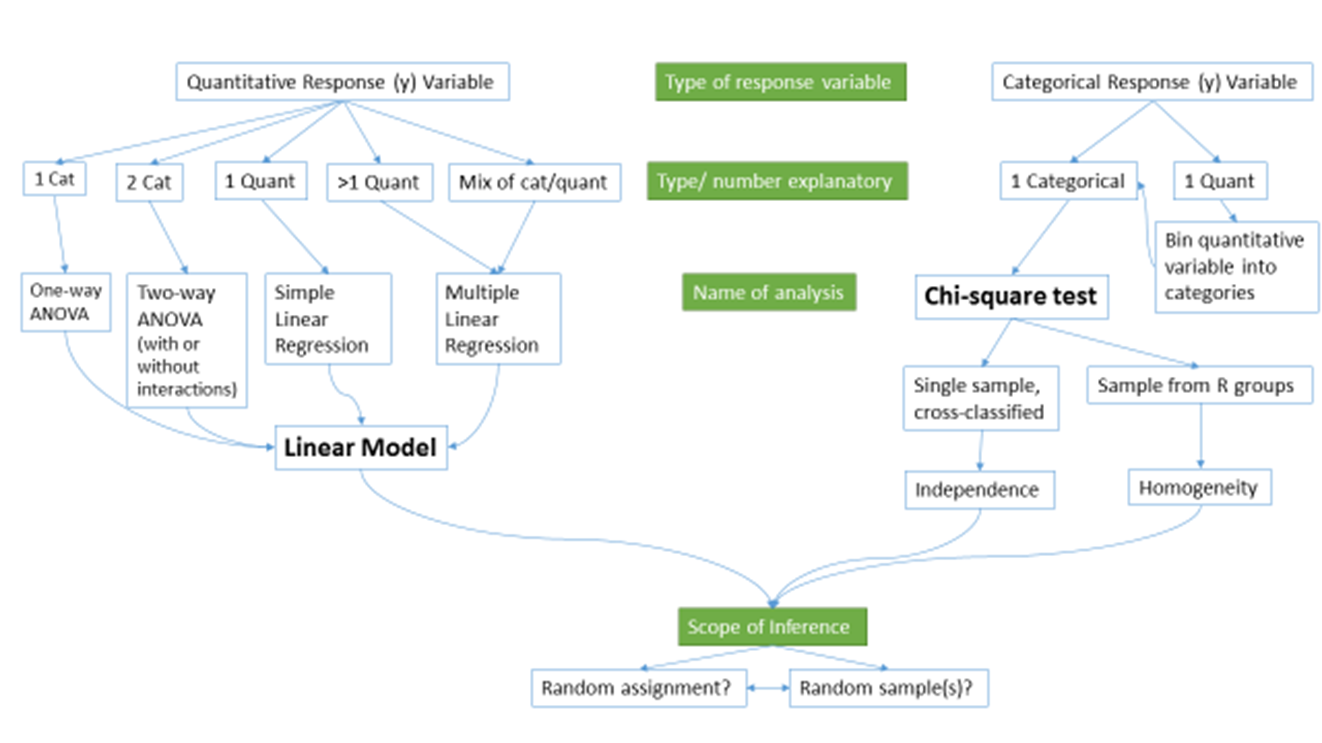
\includegraphics[width=18.36in]{chapter1_files/image002} \caption{Flow chart of methods.}\label{fig:Figure1-1}
\end{figure}

\indent We will be spending most of the semester working on methods for quantitative
response variables (the
left side of Figure \ref{fig:Figure1-1} is covered in Chapters \ref{chapter2},
\ref{chapter3}, \ref{chapter4}, \ref{chapter6}, \ref{chapter7}, and
\ref{chapter8}), stepping
over to handle the situation with a categorical response variable in Chapter \ref{chapter5} (right side
of Figure \ref{fig:Figure1-1}).
Chapter \ref{chapter9} contains case studies
illustrating all the methods discussed previously, providing a final opportunity
to explore additional examples that illustrate how finding a
path through Figure \ref{fig:Figure1-1} can lead to the appropriate analysis.

\indent The first topics (Chapters \ref{chapter1}, and \ref{chapter2}) will be more
familiar as we start with single and two group situations
with a quantitative response. In your previous statistics course, you should
have seen methods for estimating and quantifying uncertainty for the mean of a
single group and for differences in the means of two groups. Once we have briefly
reviewed these methods and introduced the statistical software that we will use
throughout the course, we will consider the first new statistical material in
Chapter \ref{chapter3}. It involves the situation with a quantitative response
variable where
there are more than 2 groups to compare -- this is what we call the \textbf{\emph{One-Way
ANOVA}} situation. It generalizes the 2-independent sample hypothesis
test to handle situations where more than 2 groups are being studied. When we
learn this method, we will begin discussing model assumptions \index{assumptions} and methods for
assessing those assumptions that will be present in every analysis involving a
quantitative response. The \textbf{\emph{Two-Way ANOVA}} (Chapter \ref{chapter3})
considers situations with two categorical explanatory variables and a
quantitative response. To make
this somewhat concrete, suppose we are interested in assessing differences in,
say, the \emph{yield} of wheat from a field based on the amount of \emph{fertilizer} applied
(none, low, or high) and \emph{variety} of wheat (two types). Here, \emph{yield} is a quantitative response variable that might be measured in bushels per acre and
there are two categorical explanatory variables, \emph{fertilizer}, with 3 levels, and \emph{variety}, with two levels. In this material, we introduce the idea of an
\textbf{\emph{interaction}} between the two explanatory variables: \index{interaction!Two-Way ANOVA} the relationship between one categorical
variable and the mean of the response changes depending on the levels of the
other categorical variable. For example, extra fertilizer might enhance the
growth of one variety and hinder the growth of another so we would say that \emph{fertilizer} has different impacts based on the level of \emph{variety}. Given this interaction may or may not actually be present, we will consider two versions of the model in Two-Way ANOVAs, \index{model!Two-Way ANOVA} what are called the \textbf{\emph{additive}} \index{model!additive} (no interaction) and the \textbf{\emph{interaction}} \index{model!interaction} models.

\indent Following the methods for two categorical variables and a quantitative response, we explore a method for
analyzing data where the response is categorical, called the \textbf{\emph{Chi-square test}}
in Chapter \ref{chapter5}. This most closely matches the One-Way ANOVA
situation with a single categorical explanatory variable, except now the
response variable is categorical. For example, we will assess whether taking a
drug (vs taking a \textbf{\emph{placebo}}\footnote{A \textbf{\emph{placebo}} is a treatment level designed to
  mimic the potentially efficacious level(s) but that can have no actual effect. The
  \textbf{\emph{placebo effect}} is the effect that thinking that an effective treatment was
  received has on subjects. There are other related issues in performing experiments
  like the \textbf{\emph{Hawthorne}} or \textbf{\emph{observer effect}} where subjects modify behavior
  because they are being observed.})
has an \textbf{\emph{effect}}\footnote{We will reserve the term ``effect'' for situations where we could
  potentially infer causal impacts on the response of the explanatory variable which
  occurs in situations where the levels of the explanatory variable are randomly
  assigned to the subjects.} on the type of improvement the subjects demonstrate. There
are two different scenarios
for study design that impact the analysis technique and hypotheses tested in
Chapter \ref{chapter5}. If the explanatory variable reflects the group that
subjects were
obtained from, either through randomization of the treatment level to the
subjects or by taking samples from separate populations, this is called a
\textbf{\emph{Chi-square Homogeneity Test}}. \index{Chi-Square Test!Homogeneity Test} It is also possible to obtain a single sample
from a population and then obtain information on the levels of the explanatory
variable for each
subject. We will analyze these results using what is called a \textbf{\emph{Chi-square Independence Test}}.
\index{Chi-Square Test!Independence Test} They both use the same test statistic but we use slightly different graphics and are testing different hypotheses in these two related
situations. Figure \ref{fig:Figure1-1} also shows that if we had a quantitative explanatory
variable and a categorical response that we would need to ``bin'' or create
categories of responses from the quantitative variable to use the Chi-square
testing methods.

\indent If the predictor and response variables are both quantitative, we start with
scatterplots, correlation,
and \textbf{\emph{simple linear regression}} models (Chapters \ref{chapter6} and
\ref{chapter7}) -- things you should have seen, at least to some degree,
previously. The biggest differences here will be
the depth of exploration of diagnostics and inferences for this model and
discussions of transformations of variables. \index{transformation} If there is more than one
explanatory variable, then we say that we are doing \textbf{\emph{multiple linear regression}}
(Chapter \ref{chapter8}) -- the ``multiple'' part of the name reflects that there will
be more
than one explanatory variable. We use the same name if we have a mix of
categorical and quantitative predictor variables but there are some new issues
in setting up the models and interpreting the coefficients that we need to
consider. In the situation with one categorical predictor and one quantitative
predictor, we revisit the idea of an interaction.
\index{interaction!MLR}
It allows us to consider situations
where the estimated relationship between a quantitative predictor and the
mean response
varies among different levels of the categorical variable.

\indent By the end of Chapter \ref{chapter9} you should be able to identify, perform
using the statistical software R \citep{R-base}, and interpret the results from each of these methods. There
is a lot to learn, but many of the tools for using R and interpreting results
of the analyses accumulate and repeat during the semester. If you work hard to
understand the initial methods, it will help you when the methods get more
complicated. You will likely feel like you are just starting to learn how to
use R at the end of the semester and for learning a new language that is
actually an accomplishment. We will just be taking you on the first steps of a
potentially long journey and it is up to you to decide how much further you
want to go with learning the software.

\indent All the methods you will learn require you to carefully consider how the data were collected, how that
pertains to the population of interest, and how that impacts the inferences
that can be made. The \textbf{\emph{scope of inference}} from the bottom of Figure
\ref{fig:Figure1-1} is our shorthand term for remembering to think about two aspects
of the study -- \textbf{\emph{random assignment}} and \textbf{\emph{random sampling}}.
\index{random assignment} \index{random sampling} In a given
situation, you need to use the description of the study to decide if the
explanatory variable was randomly assigned to study units (this allows for \textbf{\emph{causal inferences}} \index{causal effect} if differences are detected) or not (so no causal statements
are possible). As an example, think about two studies, one where students are
randomly assigned to either get tutoring with their statistics course or not
and another where the students are asked at the end of the semester whether
they sought out tutoring or not. Suppose we compare the final grades in the
course for the two groups (tutoring/not) and find a big difference. In the
first study with random assignment, \index{random assignment} we can say the tutoring caused the
differences we observed. In the second, we could only say that the tutoring was
associated with differences but because students self-selected the group they
ended up in, we can't say that the tutoring caused the differences. The other
aspect of scope of inference concerns random sampling: \index{random sampling}If the data were obtained
using a random sampling mechanism, then our inferences can be safely extended
to the population that the sample was taken from. However, if we have a non-random
sample, our inference can only apply to the sample collected. In the previous
example, the difference would be studying a random sample of students from the
population of, say, Introductory Statistics students at a university vs
studying a sample of students that volunteered for the research project, maybe
for extra credit in the class. We could still randomly assign them to
tutoring/not but the non-random sample would only lead to conclusions about
those students that volunteered. The most powerful scope of inference is when there
are randomly assigned levels of explanatory variables with a random sample from
a population -- conclusions would be about causal impacts that would happen in the
population.

\indent By the end of this material, you should have some basic R skills and abilities to create basic ANOVA and
Regression models, as well as to handle Chi-square testing situations.
Together, this should prepare you for future statistics courses or for other
situations where you are expected to be able to identify an appropriate
analysis, do the calculations for a given data set, and then effectively
communicate interpretations for the methods discussed here.

\hypertarget{section1-2}{%
\section{Getting started in R}\label{section1-2}}

You will need to download the statistical software package called R and an enhanced interface to R called
RStudio \citep{RStudio}. They are open source and free to download and use
(and will always be that way). This means that the skills you learn now can
follow you the rest of your life. R is becoming the primary language of
statistics and is being adopted across academia, government, and businesses to
help manage and learn from the growing volume of data being obtained. Hopefully
you will get a sense of some of the power of R in this book.

\indent The next pages will walk you through the process of getting the software downloaded and provide you with
an initial experience using RStudio to do things that should look familiar
even though the interface will be a new experience. Do not expect to master R
quickly -- it takes years (sorry!) even if you know the statistical methods
being used. We will try to keep all your interactions with R code in a similar
code format and that should help you in learning how to use R as we move
through various methods. We will also usually provide you with example code. Everyone
that learns R starts with copying other people's code and then making changes
for specific applications -- so expect to go back to examples from the text and focus
on learning how to modify that code to work for your particular data set. Only
really experienced R users ``know'' functions without having to check other
resources. After we complete this basic introduction, Chapter \ref{chapter2} begins doing
more sophisticated things with R, allowing us to compare quantitative responses
from two groups, make some graphical displays, do hypothesis testing \index{hypothesis testing} and create
confidence intervals in a couple of different ways.

\indent You will have two downloading activities to complete before you can do anything
more than read this book\footnote{I recorded a video that walks through getting R and RStudio installed on a PC available in the digital version \href{https://montana.techsmithrelay.com/J1Ww}{\textbf{here}}. If you want to see them installed on a mac, you can try \href{https://www.youtube.com/watch?v=GFImMj1lMRI}{\textbf{this version}}. Or for either version, try searching YouTube for ``How to install R and RStudio''.}. First, you need to download R. It is the engine that will do all the computing
for us, but you will only interact with it once. Go to \url{http://cran.rstudio.com}
and click on the ``\textbf{Download R for\ldots{}}'' button that
corresponds to your operating system. On the next page, click on ``\textbf{base}'' and then it will take you
to a screen to download the most current version of R that is compiled for your
operating system, something like ``\textbf{Download R 3.5.1 for Windows}''. Click on that link and then open
the file you downloaded. You will need to select your preferred language (choose English so your instructor can help you), then hit ``\textbf{Next}''
until it starts to unpack and install the program (all the base settings will be fine). After you hit ``\textbf{Finish}'' you will not do anything further with R directly.

\indent Second, you need to download RStudio. It is an enhanced interface that will make interacting with
R less frustrating. To download RStudio, go near the bottom of \url{https://www.rstudio.com/products/rstudio/download/} and select the correct version under
``Installers for Supported Platforms'' for your operating system. Download and
then install RStudio using the installer. From this point forward, you should only
open RStudio; it provides your interface with R. Note that both R and RStudio
are updated frequently (up to four times a year) and if you downloaded either
more than a few months previously, you should download the up-to-date versions,
especially if something you are trying to do is not working. Sometimes code
will not work in older versions of R and sometimes old code won't work in new
versions of R.\footnote{The need to keep the code up-to-date as R continues to evolve is one reason that this book is locally published and that this is the 5\textsuperscript{th} version in
  five years\ldots{}}

\indent To get started, we can complete some basic tasks in R using the RStudio
interface. When you open RStudio, you will see a screen like Figure
\ref{fig:Figure1-2}. The
added annotation in this and the following screen-grabs is there to help you
get initially oriented to the software interface. R is command-line software --
meaning that most of the time you have to create code and then enter and execute
it at a command prompt to get any results. RStudio makes the management and
execution of that code more efficient than the basic version of R. In RStudio,
the lower left panel is called the ``console'' window and is where you can type R
code directly into R or where you will see the code you run and (most
importantly!) where the results of your executed commands will show up. The
most basic interaction with R is available once you get the cursor active at
the command prompt ``\textgreater{}'' by clicking in that panel (look for a blinking
vertical line). The upper left panel is for writing, saving, and running your R
code. Once you have code available in this window, the ``Run'' button will
execute the code for the line that your cursor is on or for any text that you
have highlighted with your mouse. The ``data management'' or environment panel is
in the upper right, providing information on what data sets have been loaded.
It also contains the ``Import Dataset'' button that provides the easiest way for
you to read a data set into R so you can analyze it. The lower right panel
contains information on the ``Packages'' (additional code we will download and
install to add functionality to R) that are available and is where you will see
plots that you make and requests for ``Help'' on specific functions.



\begin{figure}[ht]
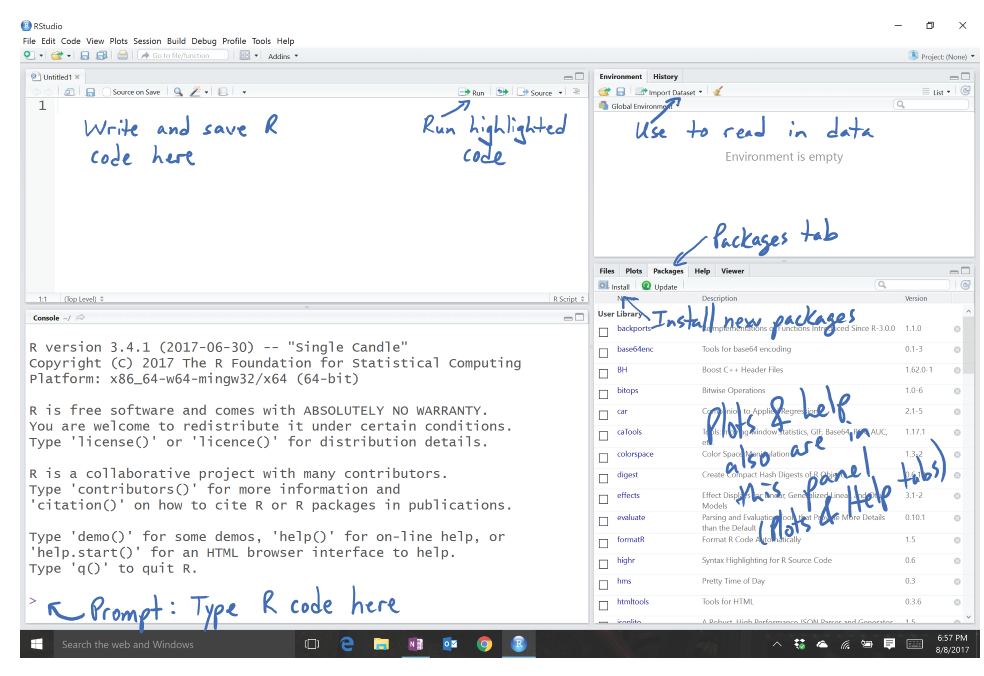
\includegraphics[width=13.67in]{chapter1_files/fig1.2} \caption{Initial RStudio layout.}\label{fig:Figure1-2}
\end{figure}

\indent As a first interaction with R we can use it as a calculator. To do this, click near the command prompt
(\texttt{\textgreater{}}) in the lower left ``console'' panel, type 3+4, and then hit enter. It
should look like this:

\begin{Shaded}
\begin{Highlighting}[]
\OperatorTok{>}\StringTok{ }\DecValTok{3}\OperatorTok{+}\DecValTok{4}
\NormalTok{[}\DecValTok{1}\NormalTok{] }\DecValTok{7}
\end{Highlighting}
\end{Shaded}

You can do more interesting calculations, like finding the mean of the
numbers -3, 5, 7, and 8 by adding them up and dividing by 4:

\begin{Shaded}
\begin{Highlighting}[]
\OperatorTok{>}\StringTok{ }\NormalTok{(}\OperatorTok{-}\DecValTok{3}\OperatorTok{+}\DecValTok{5}\OperatorTok{+}\DecValTok{7}\OperatorTok{+}\DecValTok{8}\NormalTok{)}\OperatorTok{/}\DecValTok{4}
\NormalTok{[}\DecValTok{1}\NormalTok{] }\FloatTok{4.25}
\end{Highlighting}
\end{Shaded}

Note that the parentheses help R to figure out your desired order of operations. If you drop that grouping, you get
a very different (and wrong!) result:

\begin{Shaded}
\begin{Highlighting}[]
\OperatorTok{>}\StringTok{ }\DecValTok{-3}\OperatorTok{+}\DecValTok{5}\OperatorTok{+}\DecValTok{7}\OperatorTok{+}\DecValTok{8}\OperatorTok{/}\DecValTok{4}
\NormalTok{[}\DecValTok{1}\NormalTok{] }\DecValTok{11}
\end{Highlighting}
\end{Shaded}

We could estimate the standard deviation similarly using the formula you might remember from introductory
statistics, but that will only work in very limited situations. To use the real
power of R this semester, we need to work with data sets that store the
observations for our subjects in \emph{variables}.
Basically, we need to store observations in named vectors (one dimensional
arrays) that contain a list of the observations. To create a vector containing
the four numbers and assign it to a variable named \emph{variable1}, we need to
create a vector using the function
\texttt{c} which means ``combine the items'' that follow, if they are inside
parentheses and have commas separating the values,
as follows:

\begin{Shaded}
\begin{Highlighting}[]
\OperatorTok{>}\StringTok{ }\KeywordTok{c}\NormalTok{(}\OperatorTok{-}\DecValTok{3}\NormalTok{, }\DecValTok{5}\NormalTok{, }\DecValTok{7}\NormalTok{, }\DecValTok{8}\NormalTok{)}
\NormalTok{[}\DecValTok{1}\NormalTok{] }\DecValTok{-3} \DecValTok{5} \DecValTok{7} \DecValTok{8}
\end{Highlighting}
\end{Shaded}

To get this vector stored in a variable called \emph{variable1} we need to
use the assignment operator, \texttt{\textless{}-} (read as ``is defined to contain'') that assigns
the information on the right into the variable that you are creating on
the left.

\begin{Shaded}
\begin{Highlighting}[]
\OperatorTok{>}\StringTok{ }\NormalTok{variable1 <-}\StringTok{ }\KeywordTok{c}\NormalTok{(}\OperatorTok{-}\DecValTok{3}\NormalTok{, }\DecValTok{5}\NormalTok{, }\DecValTok{7}\NormalTok{, }\DecValTok{8}\NormalTok{)}
\end{Highlighting}
\end{Shaded}

In R, the assignment operator, \texttt{\textless{}-}, is created by typing a
``less than'' symbol \texttt{\textless{}} followed by a ``minus'' sign (\texttt{-})
\textbf{without a space between them}. If you
ever want to see what numbers are residing in an object in R, just type
its name and hit \emph{enter}. You can see how that variable contains the same
information that was initially generated by
\texttt{c(-3,\ 5,\ 7,\ 8)} but is easier to access since we just need the text
for the variable name representing that vector.

\begin{Shaded}
\begin{Highlighting}[]
\OperatorTok{>}\StringTok{ }\NormalTok{variable1}
\NormalTok{[}\DecValTok{1}\NormalTok{] }\DecValTok{-3} \DecValTok{5} \DecValTok{7} \DecValTok{8}
\end{Highlighting}
\end{Shaded}

With the data stored in a variable, we can use functions such as
\texttt{mean} and
\texttt{sd} to find the mean and standard deviation of the observations contained in
\texttt{variable1}:
\index{mean}
\index{standard deviation}

\begin{Shaded}
\begin{Highlighting}[]
\OperatorTok{>}\StringTok{ }\KeywordTok{mean}\NormalTok{(variable1)}
\NormalTok{[}\DecValTok{1}\NormalTok{] }\FloatTok{4.25}
\OperatorTok{>}\StringTok{ }\KeywordTok{sd}\NormalTok{(variable1)}
\NormalTok{[}\DecValTok{1}\NormalTok{] }\FloatTok{4.99166}
\end{Highlighting}
\end{Shaded}

\indent When dealing with real data, we will often have information about more than one
variable. We could enter all observations by hand for each variable but this is
prone to error and onerous for all but the smallest data sets. If you are to
ever utilize the power of statistics in the evolving data-centered world, data
management has to be accomplished in a more sophisticated way. While you can
manage data sets quite effectively in R, it is often easiest to start with your
data set in something like Microsoft Excel or OpenOffice's Calc. You want to
make sure that observations are in the rows and the names of variables are in
the columns and that there is no ``extra stuff'' in the spreadsheet. If you have
missing observations, they should be represented with blank cells. The file should
be saved as a ``.csv'' file (stands for comma-separated values although Excel
calls it ``CSV (Comma Delimited)''), which basically strips off some of the junk
that Excel adds to the necessary information in the file. Excel will tell you that
this is a bad idea, but it actually creates a more stable archival format and
one that R can use directly.\footnote{There are ways to read ``.xls'' and ``.xlsx'' files
  directly into R that we will explore later.}

\indent The following code to read in the data set relies on an R package called
\texttt{readr} \citep{R-readr}. Packages in R provide additional functions and data sets that
are not available in the initial download of R or RStudio. To get access to the packages,
first ``install'' (basically
download) and then ``load'' the package. To install an R package, go to the \textbf{Packages}
tab in the lower right panel of
RStudio. Click on the \textbf{Install} button and then type in the name of the package in
the box (here type in \texttt{readr}).
\index{R packages!\textbf{readr}}
RStudio will try to auto-complete the package name
you are typing which should help you make sure you got it typed correctly. This will
be the first of \emph{many} times that we will mention that R is case sensitive -- in
other words, \texttt{Readr} is different from \texttt{readr} in R syntax and this sort of
thing applies to everything you do in R. You should only need to install each R
package once on a given computer. If you ever see a message that R can't find a
package, make sure it appears in the list in the \textbf{Packages} tab. If it
doesn't, repeat the previous steps to install it.

\begin{longtable}[]{@{}l@{}}
\toprule
\endhead
\textbf{Important}: R is case sensitive! \texttt{Readr} is not the same as \texttt{readr}!\tabularnewline
\bottomrule
\end{longtable}

\indent After installing the package, we need to load it to make it active in a given work
session. Go to the command prompt and type (or copy and paste) \texttt{require(readr)} or \texttt{library(readr)}:
\index{R packages!\textbf{readr}}

\begin{verbatim}
> require(readr)
\end{verbatim}

With a data set converted to a CSV file and \texttt{readr} installed and loaded, we need to read the data set into the active workspace.
\index{import data}
There are two ways to do this, either using the point-and-click GUI in RStudio (click
the ``Import Dataset'' button in the upper right ``Environment'' panel as
indicated in Figure \ref{fig:Figure1-2}) or modifying the \texttt{read\_csv}
function to find the file of interest. To practice this, you can
download an Excel (.xls) file from
\url{http://www.math.montana.edu/courses/s217/documents/treadmill.xls}
that contains observations on 31 males that volunteered for a study on methods
for measuring fitness \citep{Westfall1993}.
In the spreadsheet, you will find a data set that
starts and ends with the following information (only results for Subjects 1, 2,
30, and 31 shown here):

\begin{longtable}[]{@{}lllrrlrr@{}}
\toprule
\begin{minipage}[b]{0.07\columnwidth}\raggedright
Sub-
ject\strut
\end{minipage} & \begin{minipage}[b]{0.10\columnwidth}\raggedright
Tread-
MillOx\strut
\end{minipage} & \begin{minipage}[b]{0.13\columnwidth}\raggedright
TreadMill-
MaxPulse\strut
\end{minipage} & \begin{minipage}[b]{0.09\columnwidth}\raggedleft
RunTime\strut
\end{minipage} & \begin{minipage}[b]{0.10\columnwidth}\raggedleft
RunPulse\strut
\end{minipage} & \begin{minipage}[b]{0.08\columnwidth}\raggedright
Rest
Pulse\strut
\end{minipage} & \begin{minipage}[b]{0.14\columnwidth}\raggedleft
BodyWeight\strut
\end{minipage} & \begin{minipage}[b]{0.05\columnwidth}\raggedleft
Age\strut
\end{minipage}\tabularnewline
\midrule
\endhead
\begin{minipage}[t]{0.07\columnwidth}\raggedright
1\strut
\end{minipage} & \begin{minipage}[t]{0.10\columnwidth}\raggedright
60.05\strut
\end{minipage} & \begin{minipage}[t]{0.13\columnwidth}\raggedright
186\strut
\end{minipage} & \begin{minipage}[t]{0.09\columnwidth}\raggedleft
8.63\strut
\end{minipage} & \begin{minipage}[t]{0.10\columnwidth}\raggedleft
170\strut
\end{minipage} & \begin{minipage}[t]{0.08\columnwidth}\raggedright
48\strut
\end{minipage} & \begin{minipage}[t]{0.14\columnwidth}\raggedleft
81.87\strut
\end{minipage} & \begin{minipage}[t]{0.05\columnwidth}\raggedleft
38\strut
\end{minipage}\tabularnewline
\begin{minipage}[t]{0.07\columnwidth}\raggedright
2\strut
\end{minipage} & \begin{minipage}[t]{0.10\columnwidth}\raggedright
59.57\strut
\end{minipage} & \begin{minipage}[t]{0.13\columnwidth}\raggedright
172\strut
\end{minipage} & \begin{minipage}[t]{0.09\columnwidth}\raggedleft
8.17\strut
\end{minipage} & \begin{minipage}[t]{0.10\columnwidth}\raggedleft
166\strut
\end{minipage} & \begin{minipage}[t]{0.08\columnwidth}\raggedright
40\strut
\end{minipage} & \begin{minipage}[t]{0.14\columnwidth}\raggedleft
68.15\strut
\end{minipage} & \begin{minipage}[t]{0.05\columnwidth}\raggedleft
42\strut
\end{minipage}\tabularnewline
\begin{minipage}[t]{0.07\columnwidth}\raggedright
\ldots{}\strut
\end{minipage} & \begin{minipage}[t]{0.10\columnwidth}\raggedright
\ldots{}\strut
\end{minipage} & \begin{minipage}[t]{0.13\columnwidth}\raggedright
\ldots{}\strut
\end{minipage} & \begin{minipage}[t]{0.09\columnwidth}\raggedleft
\ldots{}\strut
\end{minipage} & \begin{minipage}[t]{0.10\columnwidth}\raggedleft
\ldots{}\strut
\end{minipage} & \begin{minipage}[t]{0.08\columnwidth}\raggedright
\ldots{}\strut
\end{minipage} & \begin{minipage}[t]{0.14\columnwidth}\raggedleft
\ldots{}\strut
\end{minipage} & \begin{minipage}[t]{0.05\columnwidth}\raggedleft
\ldots{}\strut
\end{minipage}\tabularnewline
\begin{minipage}[t]{0.07\columnwidth}\raggedright
30\strut
\end{minipage} & \begin{minipage}[t]{0.10\columnwidth}\raggedright
39.2\strut
\end{minipage} & \begin{minipage}[t]{0.13\columnwidth}\raggedright
172\strut
\end{minipage} & \begin{minipage}[t]{0.09\columnwidth}\raggedleft
12.88\strut
\end{minipage} & \begin{minipage}[t]{0.10\columnwidth}\raggedleft
168\strut
\end{minipage} & \begin{minipage}[t]{0.08\columnwidth}\raggedright
44\strut
\end{minipage} & \begin{minipage}[t]{0.14\columnwidth}\raggedleft
91.63\strut
\end{minipage} & \begin{minipage}[t]{0.05\columnwidth}\raggedleft
54\strut
\end{minipage}\tabularnewline
\begin{minipage}[t]{0.07\columnwidth}\raggedright
31\strut
\end{minipage} & \begin{minipage}[t]{0.10\columnwidth}\raggedright
37.39\strut
\end{minipage} & \begin{minipage}[t]{0.13\columnwidth}\raggedright
192\strut
\end{minipage} & \begin{minipage}[t]{0.09\columnwidth}\raggedleft
14.03\strut
\end{minipage} & \begin{minipage}[t]{0.10\columnwidth}\raggedleft
186\strut
\end{minipage} & \begin{minipage}[t]{0.08\columnwidth}\raggedright
56\strut
\end{minipage} & \begin{minipage}[t]{0.14\columnwidth}\raggedleft
87.66\strut
\end{minipage} & \begin{minipage}[t]{0.05\columnwidth}\raggedleft
45\strut
\end{minipage}\tabularnewline
\bottomrule
\end{longtable}

\indent The variables contain information on the subject number (\emph{Subject}), subjects'
maximum treadmill oxygen consumption (\emph{TreadMillOx}, in ml per kg per minute, also called maximum VO2) and
maximum pulse rate (\emph{TreadMillMaxPulse}, in beats per minute), time to run 1.5
miles (\emph{Run Time}, in minutes), maximum pulse
during 1.5 mile run (\emph{RunPulse}, in beats per minute), resting pulse rate
(\emph{RestPulse}, beats per minute), Body Weight (\emph{BodyWeight}, in kg), and \emph{Age}
(in years). Open the file in Excel or equivalent software and then save it as
a .csv file in a location you can find on your computer. Then go to RStudio
and click on \textbf{File}, then \textbf{Import Dataset}, then \textbf{From Text (readr)\ldots{}}\footnote{If
  you are having trouble getting the file converted and read into R, copy and
  run the following code:
  \texttt{treadmill\ \textless{}-\ read\_csv("http://www.math.montana.edu/courses/s217/documents/treadmill.csv")}.}
\index{import data}
Find your file and click ``\textbf{Import}''. R will store the data set as an object with the same name
as the .csv file. You could use another name as well, but it is
often easiest just to keep the data
set name in R related to the original file name. You should see some text appear
in the console (lower left panel) like in Figure \ref{fig:Figure1-3}. The text
that is created
will look something like the following -- if you had stored the file in a drive
labeled D:, it would be:

\begin{Shaded}
\begin{Highlighting}[]
\NormalTok{treadmill <-}\StringTok{ }\KeywordTok{read_csv}\NormalTok{(}\StringTok{"D:/treadmill.csv"}\NormalTok{)}
\end{Highlighting}
\end{Shaded}

What is put inside the
\texttt{"\ "} will depend on the location and name of your saved .csv file. A
version of the data set in what looks like a
spreadsheet will appear in the upper left window due to the second line of
code (\texttt{View(treadmill})).



\begin{figure}[ht]
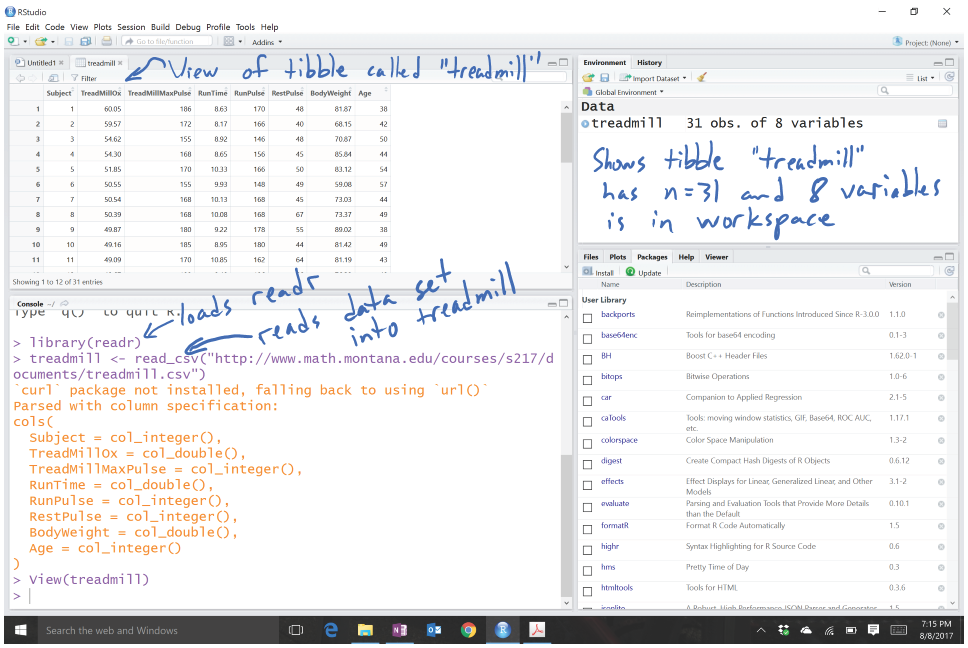
\includegraphics[width=13.44in]{chapter1_files/fig1.3} \caption{RStudio with initial data set loaded.}\label{fig:Figure1-3}
\end{figure}

\indent Just directly typing (or using) a line of code like this is actually the
other way that we can read in
files. If you choose to use the text-only interface, then you need to tell R
where to look in your computer to find the data file. \texttt{read\_csv} is a
function that takes a path as an argument. To use it, specify the path to
your data file, put quotes around it, and put it as the input to
\texttt{read\_csv(...)}. For some examples later in the book, you will be able to
copy a command like this from the text and read data sets and other
code directly from the course folder, assuming you are connected to the
internet.

\indent To verify that you read the data set in correctly, it is always good to check
its contents. We can view the first and last rows in the data set using the
\texttt{head} and \texttt{tail} functions on the data set, which show the following
results for the
\texttt{treadmill} data. Note that you will sometimes need to resize the console
window in RStudio to get all the columns to display
in a single row which can be performed by dragging the gray bars that separate
the panels.
\index{\texttt{head()}}
\index{\texttt{tail()}}

\small

\begin{Shaded}
\begin{Highlighting}[]
\OperatorTok{>}\StringTok{ }\KeywordTok{head}\NormalTok{(treadmill)}
\CommentTok{# A tibble: 6 x 8}
\NormalTok{  Subject TreadMillOx TreadMillMaxPulse RunTime RunPulse RestPulse BodyWeight   Age}
    \OperatorTok{<}\NormalTok{int}\OperatorTok{>}\StringTok{       }\ErrorTok{<}\NormalTok{dbl}\OperatorTok{>}\StringTok{             }\ErrorTok{<}\NormalTok{int}\OperatorTok{>}\StringTok{   }\ErrorTok{<}\NormalTok{dbl}\OperatorTok{>}\StringTok{    }\ErrorTok{<}\NormalTok{int}\OperatorTok{>}\StringTok{     }\ErrorTok{<}\NormalTok{int}\OperatorTok{>}\StringTok{      }\ErrorTok{<}\NormalTok{dbl}\OperatorTok{>}\StringTok{ }\ErrorTok{<}\NormalTok{int}\OperatorTok{>}
\DecValTok{1}       \DecValTok{1}       \FloatTok{60.05}               \DecValTok{186}    \FloatTok{8.63}      \DecValTok{170}        \DecValTok{48}      \FloatTok{81.87}    \DecValTok{38}
\DecValTok{2}       \DecValTok{2}       \FloatTok{59.57}               \DecValTok{172}    \FloatTok{8.17}      \DecValTok{166}        \DecValTok{40}      \FloatTok{68.15}    \DecValTok{42}
\DecValTok{3}       \DecValTok{3}       \FloatTok{54.62}               \DecValTok{155}    \FloatTok{8.92}      \DecValTok{146}        \DecValTok{48}      \FloatTok{70.87}    \DecValTok{50}
\DecValTok{4}       \DecValTok{4}       \FloatTok{54.30}               \DecValTok{168}    \FloatTok{8.65}      \DecValTok{156}        \DecValTok{45}      \FloatTok{85.84}    \DecValTok{44}
\DecValTok{5}       \DecValTok{5}       \FloatTok{51.85}               \DecValTok{170}   \FloatTok{10.33}      \DecValTok{166}        \DecValTok{50}      \FloatTok{83.12}    \DecValTok{54}
\DecValTok{6}       \DecValTok{6}       \FloatTok{50.55}               \DecValTok{155}    \FloatTok{9.93}      \DecValTok{148}        \DecValTok{49}      \FloatTok{59.08}    \DecValTok{57}

\OperatorTok{>}\StringTok{ }\KeywordTok{tail}\NormalTok{(treadmill)}
\CommentTok{# A tibble: 6 x 8}
\NormalTok{  Subject TreadMillOx TreadMillMaxPulse RunTime RunPulse RestPulse BodyWeight   Age}
    \OperatorTok{<}\NormalTok{int}\OperatorTok{>}\StringTok{       }\ErrorTok{<}\NormalTok{dbl}\OperatorTok{>}\StringTok{             }\ErrorTok{<}\NormalTok{int}\OperatorTok{>}\StringTok{   }\ErrorTok{<}\NormalTok{dbl}\OperatorTok{>}\StringTok{    }\ErrorTok{<}\NormalTok{int}\OperatorTok{>}\StringTok{     }\ErrorTok{<}\NormalTok{int}\OperatorTok{>}\StringTok{      }\ErrorTok{<}\NormalTok{dbl}\OperatorTok{>}\StringTok{ }\ErrorTok{<}\NormalTok{int}\OperatorTok{>}
\DecValTok{1}      \DecValTok{26}       \FloatTok{44.61}               \DecValTok{182}   \FloatTok{11.37}      \DecValTok{178}        \DecValTok{62}      \FloatTok{89.47}    \DecValTok{44}
\DecValTok{2}      \DecValTok{27}       \FloatTok{40.84}               \DecValTok{172}   \FloatTok{10.95}      \DecValTok{168}        \DecValTok{57}      \FloatTok{69.63}    \DecValTok{51}
\DecValTok{3}      \DecValTok{28}       \FloatTok{39.44}               \DecValTok{176}   \FloatTok{13.08}      \DecValTok{174}        \DecValTok{63}      \FloatTok{81.42}    \DecValTok{44}
\DecValTok{4}      \DecValTok{29}       \FloatTok{39.41}               \DecValTok{176}   \FloatTok{12.63}      \DecValTok{174}        \DecValTok{58}      \FloatTok{73.37}    \DecValTok{57}
\DecValTok{5}      \DecValTok{30}       \FloatTok{39.20}               \DecValTok{172}   \FloatTok{12.88}      \DecValTok{168}        \DecValTok{44}      \FloatTok{91.63}    \DecValTok{54}
\DecValTok{6}      \DecValTok{31}       \FloatTok{37.39}               \DecValTok{192}   \FloatTok{14.03}      \DecValTok{186}        \DecValTok{56}      \FloatTok{87.66}    \DecValTok{45}
\end{Highlighting}
\end{Shaded}

\normalsize

\indent When you require a package, you may see a warning message about versions of the package and versions of
R -- this is \emph{usually} something you can ignore. Other warning messages could
be more ominous for proceeding but before getting too concerned, there are
couple of basic things to check.
\index{warning message}
First, double check that the package is
installed (see
previous steps). Second, check for typographical errors in your code --
especially for mis-spellings or unintended capitalization. If you are still
having issues, try repeating the installation process. If that fails, find
someone more used to using R to help you (for example in the Math Learning
Center or by emailing your instructor).\footnote{Most computer lab computers at
  Montana State University have RStudio installed and so provide another venue
  to work.}

\indent To help you go from basic to intermediate R usage and especially to help with more
complicated problems, you will want to learn how to manage and save your R code.
The best way to do this is using the upper left panel in RStudio using what
are called R Scripts, which are files that have a file extension of ``.R''. To
start a new ``.R'' file to store your code, click on \textbf{File}, then
\textbf{New File}, then \textbf{R Script}. This will create a blank page to enter and
edit code -- then save the file as something like ``MyFileName.R'' in your preferred location.
Saving your code will mean that you can return to where you
were working last by simply re-running the saved script file. With code in the
script window, you can place the cursor on a line of code or highlight a chunk
of code and hit the ``Run'' button\footnote{You can also use Ctrl+Enter if you like hot keys.}
on the upper part of the panel. It will appear
in the console with results just like what you would obtain if you typed it
after the command prompt and hit enter for each line. Figure \ref{fig:Figure1-4}
shows the screen with the code used in this
section in the upper left panel, saved in
a file called ``CH0.R'', with the results of highlighting and executing the first
section of code using the ``Run'' button.



\begin{figure}[ht]
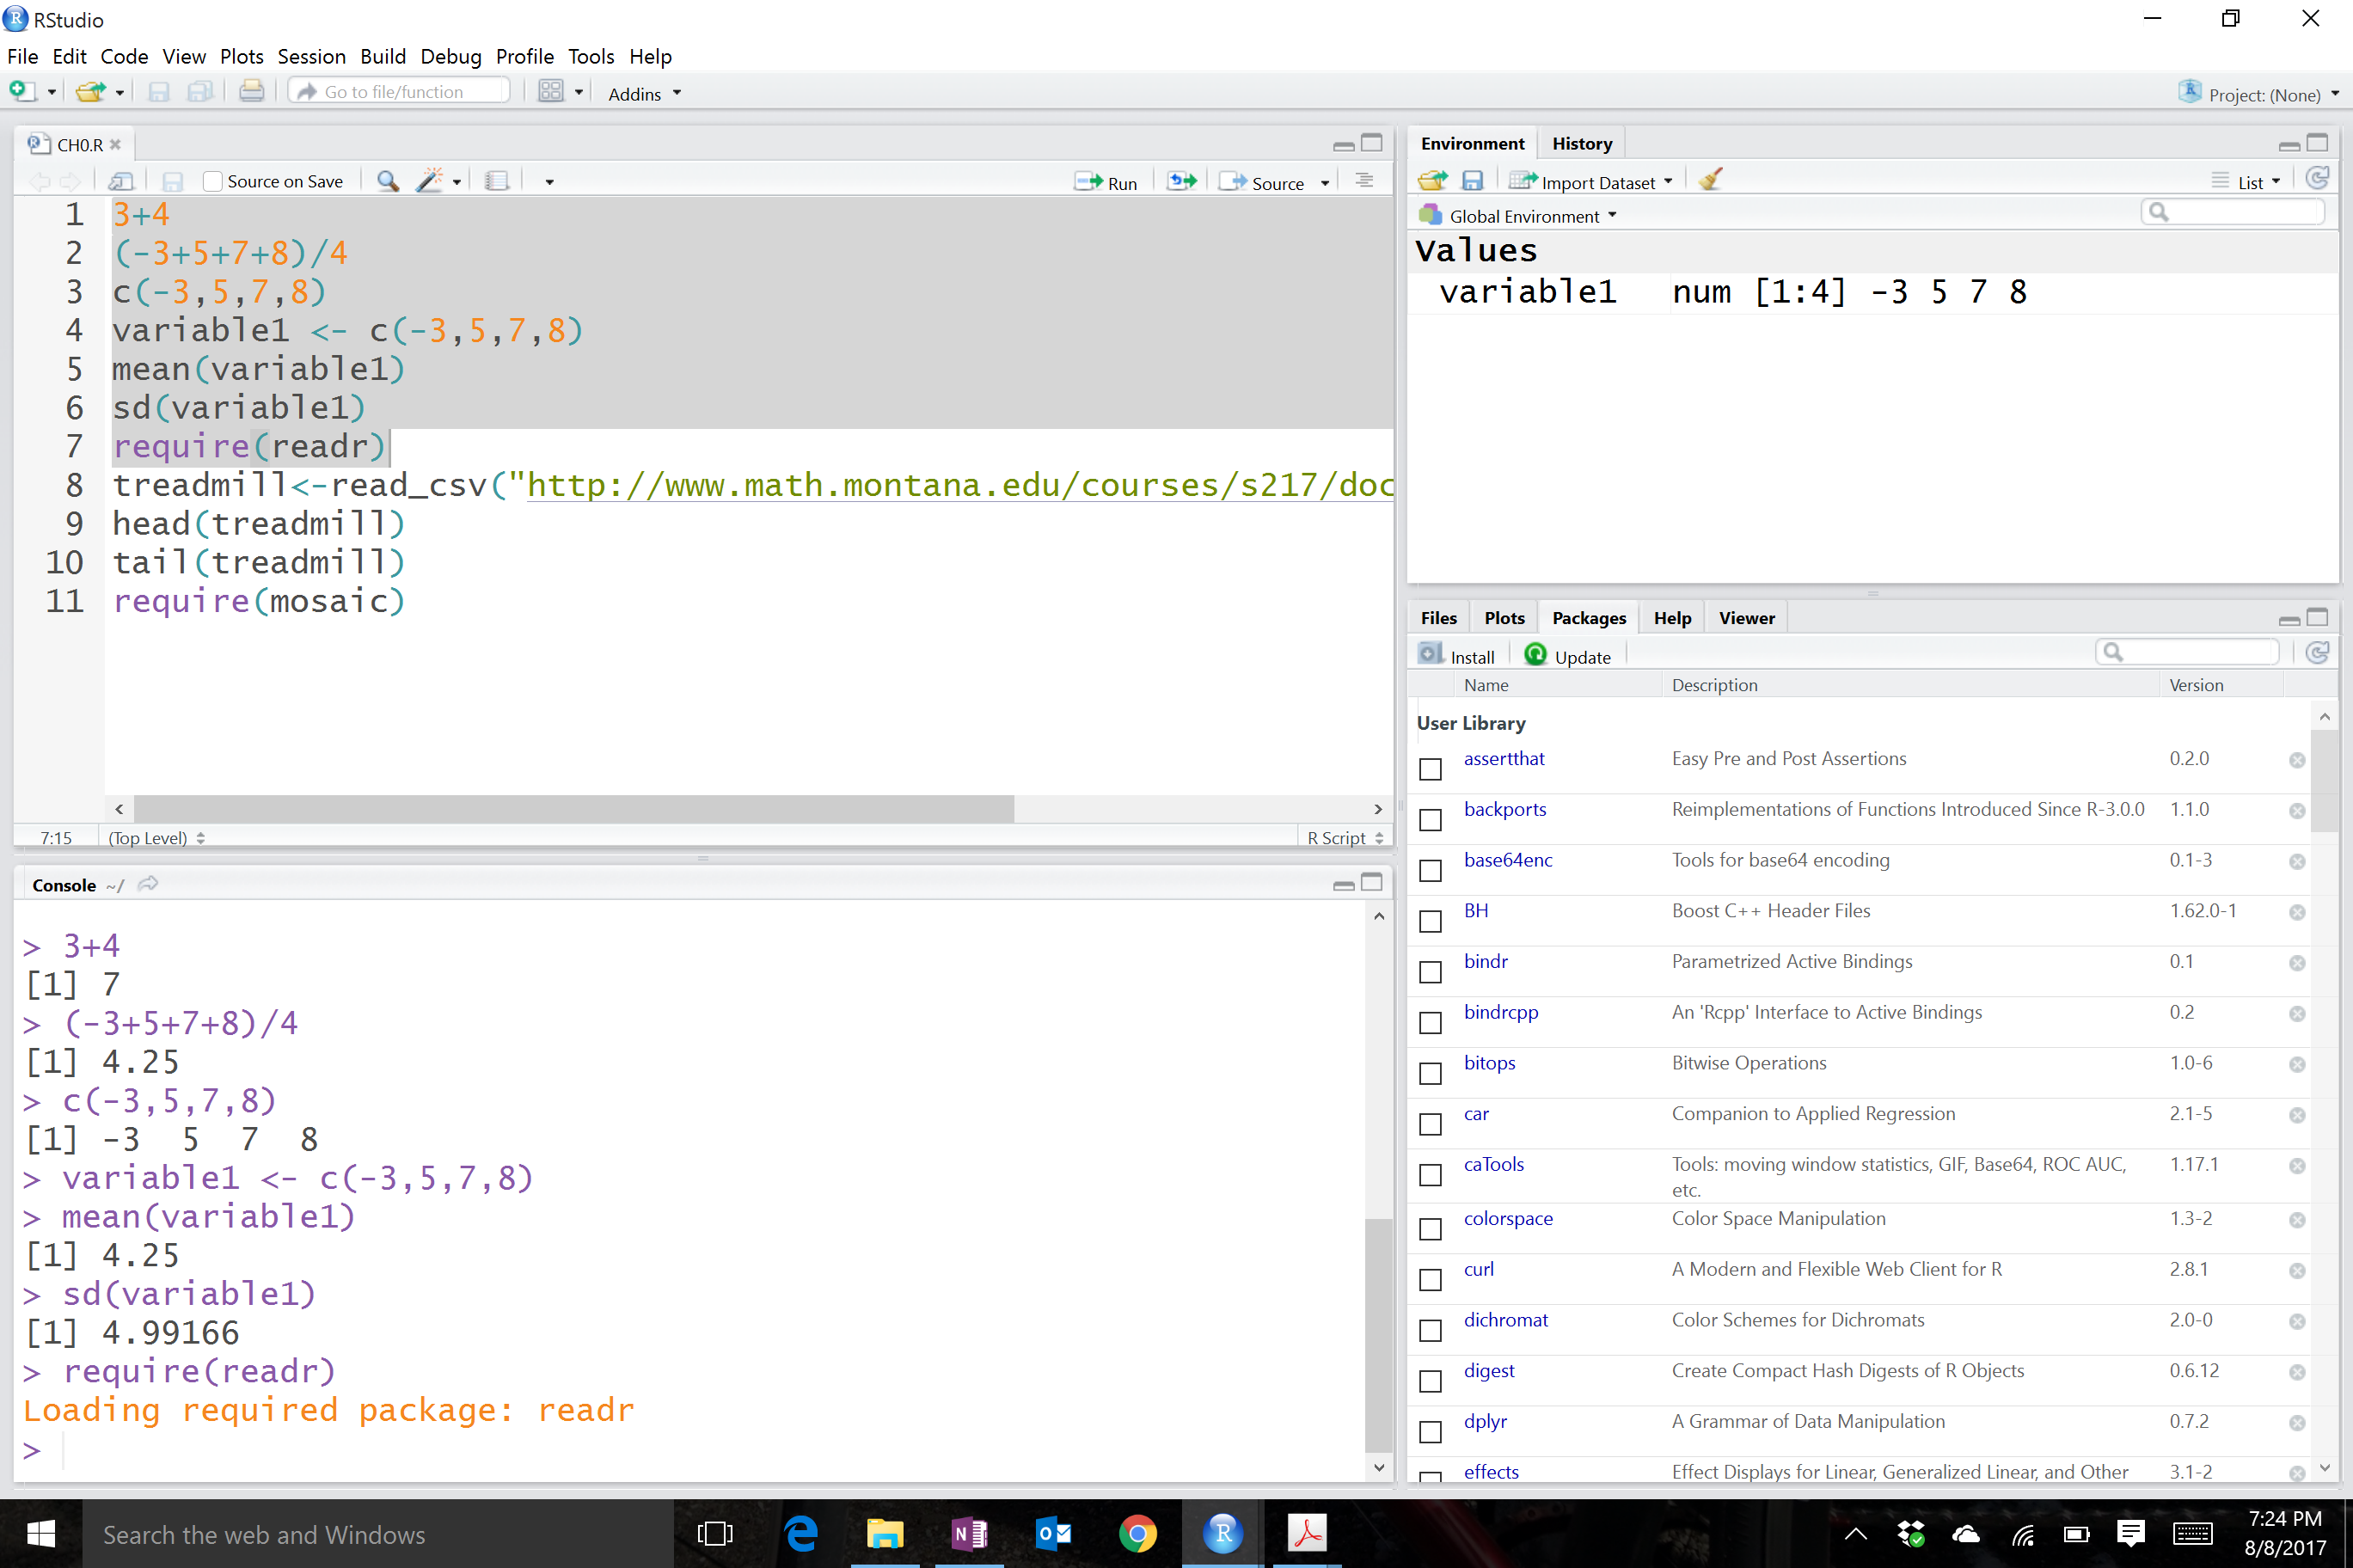
\includegraphics[width=38.01in]{chapter1_files/fig1.4} \caption{RStudio with highlighted code run.}\label{fig:Figure1-4}
\end{figure}

\hypertarget{section1-3}{%
\section{Basic summary statistics, histograms, and boxplots using R}\label{section1-3}}

For the following material, you will need to install and load the \texttt{mosaic} package \citep{R-mosaic}.

\index{R packages!\textbf{mosaic}}

\begin{Shaded}
\begin{Highlighting}[]
\OperatorTok{>}\StringTok{ }\KeywordTok{require}\NormalTok{(mosaic)}
\end{Highlighting}
\end{Shaded}

It provides a suite of enhanced functions to aid our initial explorations. With RStudio running, the \texttt{mosaic} package loaded, a place to write and
save code, and the \texttt{treadmill} data set loaded, we can (finally!) start to
summarize the results of the study. The \texttt{treadmill} object is what R calls a
\textbf{\emph{tibble}}\footnote{Tibbles are R are objects that can contain both
  categorical and quantitative variables on your \(n\) subjects with a name for each
  variable that is also the name of each column in a matrix. \index{tibble} Each subject is a
  row of the data set. The name (supposedly) is due to the way \emph{table} sounds in the accent of a particularly influential developer at RStudio who is from New Zealand.} and contains columns corresponding to each variable in
the spreadsheet. Every
function in R will involve specifying the variable(s) of interest and how you
want to use them. To access a particular variable (column) in a tibble, you
can use a \$ between the name of the tibble and the name of the variable of
interest, generically as \texttt{tibblename\$variablename}. You can think of this as \emph{tibblename's variablename} where the \emph{'s} is replaced by the dollar sign. To identify the
\texttt{RunTime} variable here it would be \texttt{treadmill\$RunTime}. In the command line it would look like:

\begin{Shaded}
\begin{Highlighting}[]
\OperatorTok{>}\StringTok{ }\NormalTok{treadmill}\OperatorTok{$}\NormalTok{RunTime}
\NormalTok{[}\DecValTok{1}\NormalTok{]  }\FloatTok{8.63}  \FloatTok{8.17}  \FloatTok{8.92}  \FloatTok{8.65} \FloatTok{10.33}  \FloatTok{9.93} \FloatTok{10.13} \FloatTok{10.08}  \FloatTok{9.22}  \FloatTok{8.95} \FloatTok{10.85}  \FloatTok{9.40} \FloatTok{11.50} \FloatTok{10.50}
\NormalTok{[}\DecValTok{15}\NormalTok{] }\FloatTok{10.60} \FloatTok{10.25} \FloatTok{10.00} \FloatTok{11.17} \FloatTok{10.47} \FloatTok{11.95}  \FloatTok{9.63} \FloatTok{10.07} \FloatTok{11.08} \FloatTok{11.63} \FloatTok{11.12} \FloatTok{11.37} \FloatTok{10.95} \FloatTok{13.08}
\NormalTok{[}\DecValTok{29}\NormalTok{] }\FloatTok{12.63} \FloatTok{12.88} \FloatTok{14.03}
\end{Highlighting}
\end{Shaded}

\indent Just as in the previous section, we can generate summary statistics using functions like \texttt{mean} and \texttt{sd} by running them on a specific variable:
\index{mean}
\index{standard deviation}

\begin{Shaded}
\begin{Highlighting}[]
\OperatorTok{>}\StringTok{ }\KeywordTok{mean}\NormalTok{(treadmill}\OperatorTok{$}\NormalTok{RunTime)}
\NormalTok{[}\DecValTok{1}\NormalTok{] }\FloatTok{10.58613}
\OperatorTok{>}\StringTok{ }\KeywordTok{sd}\NormalTok{(treadmill}\OperatorTok{$}\NormalTok{RunTime)}
\NormalTok{[}\DecValTok{1}\NormalTok{] }\FloatTok{1.387414}
\end{Highlighting}
\end{Shaded}

And now we know that the average running time for 1.5 miles for the subjects in the study was 10.6 minutes with a standard deviation (SD) of 1.39 minutes. But you should remember that the
mean and SD are only appropriate summaries if the distribution is roughly
\textbf{\emph{symmetric}} (both sides of the distribution are approximately the same shape and length). The
\texttt{mosaic} package provides a useful function called \texttt{favstats} that provides
the mean and SD as well as the \textbf{\emph{5 number summary}}: \index{5 number summary}
the minimum (\texttt{min}), the first quartile (\texttt{Q1}, the 25\textsuperscript{th} percentile),
the median (50\textsuperscript{th} percentile), the third quartile (\texttt{Q3}, the 75\textsuperscript{th}
percentile), and the maximum (\texttt{max}). It also provides the number of
observations (\texttt{n}) which was 31, as noted above, and a count of whether any
missing values were encountered (\texttt{missing}), which was 0 here since all
subjects had measurements available on this variable.
\index{favstats}

\begin{Shaded}
\begin{Highlighting}[]
\OperatorTok{>}\StringTok{ }\KeywordTok{favstats}\NormalTok{(treadmill}\OperatorTok{$}\NormalTok{RunTime)}
\NormalTok{  min   Q1 median    Q3   max     mean       sd  n missing}
 \FloatTok{8.17} \FloatTok{9.78}  \FloatTok{10.47} \FloatTok{11.27} \FloatTok{14.03} \FloatTok{10.58613} \FloatTok{1.387414} \DecValTok{31}       \DecValTok{0}
\end{Highlighting}
\end{Shaded}

\indent We are starting to get somewhere with understanding that the runners were
somewhat fit with worst runner covering 1.5 miles in 14 minutes
(the equivalent of a 9.3 minute mile)
and the best running at a 5.4 minute mile pace. The limited variation in the
results suggests that the sample was obtained from a restricted group with
somewhat common characteristics. When you explore the ages and weights of the
subjects in the Practice Problems in Section \ref{section1-6}, you will get even more
information about how similar all the subjects in this study were. Researchers often publish numerical summaries of this sort of demographic information to help readers understand the subjects that they studied and that their results might apply to.

\indent A graphical display of these results will help us to assess the shape
of the distribution of run times -- including considering the potential for the presence of a \textbf{\emph{skew}} (whether the right or left tail of the distribution
is noticeably more spread out, with left skew meaning that the left tail
is more spread out than the right tail) \index{skew} and \textbf{\emph{outliers}} \index{outlier}
(unusual observations). A \textbf{\emph{histogram}} \index{histogram} is a good place to start.
Histograms display connected bars with counts of observations defining
the height of bars based on a set of bins of values of the quantitative variable.
We will apply the \texttt{hist} function to the \texttt{RunTime} variable, which produces
Figure \ref{fig:Figure1-5}.

\begin{Shaded}
\begin{Highlighting}[]
\OperatorTok{>}\StringTok{ }\KeywordTok{hist}\NormalTok{(treadmill}\OperatorTok{$}\NormalTok{RunTime)}
\end{Highlighting}
\end{Shaded}



\begin{figure}
\centering
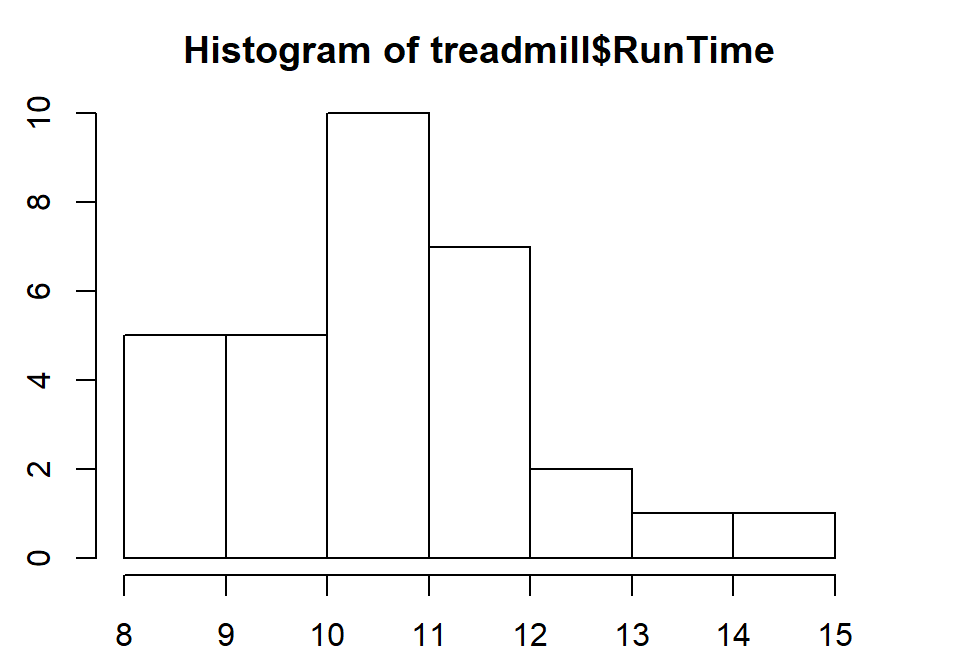
\includegraphics{01-preface_files/figure-latex/Figure1-5-1.pdf}
\caption{\label{fig:Figure1-5}Histogram of Run Times (minutes) of \(n\)=31 subjects in Treadmill study, bar heights are counts.}
\end{figure}

\indent You can save this plot by clicking on the \textbf{Export} button found above
the plot, followed by \textbf{Copy to Clipboard} and clicking on the
\textbf{Copy Plot} button. Then if you open your
favorite word-processing program, you should be able to paste it into a
document for writing reports that include the figures. You can see the first
parts of this process in the screen grab in Figure \ref{fig:Figure1-6}. You can also directly save the figures as separate files using
\textbf{Save as Image} or \textbf{Save as PDF} and then insert them into your word
processing documents.



\begin{figure}[ht]
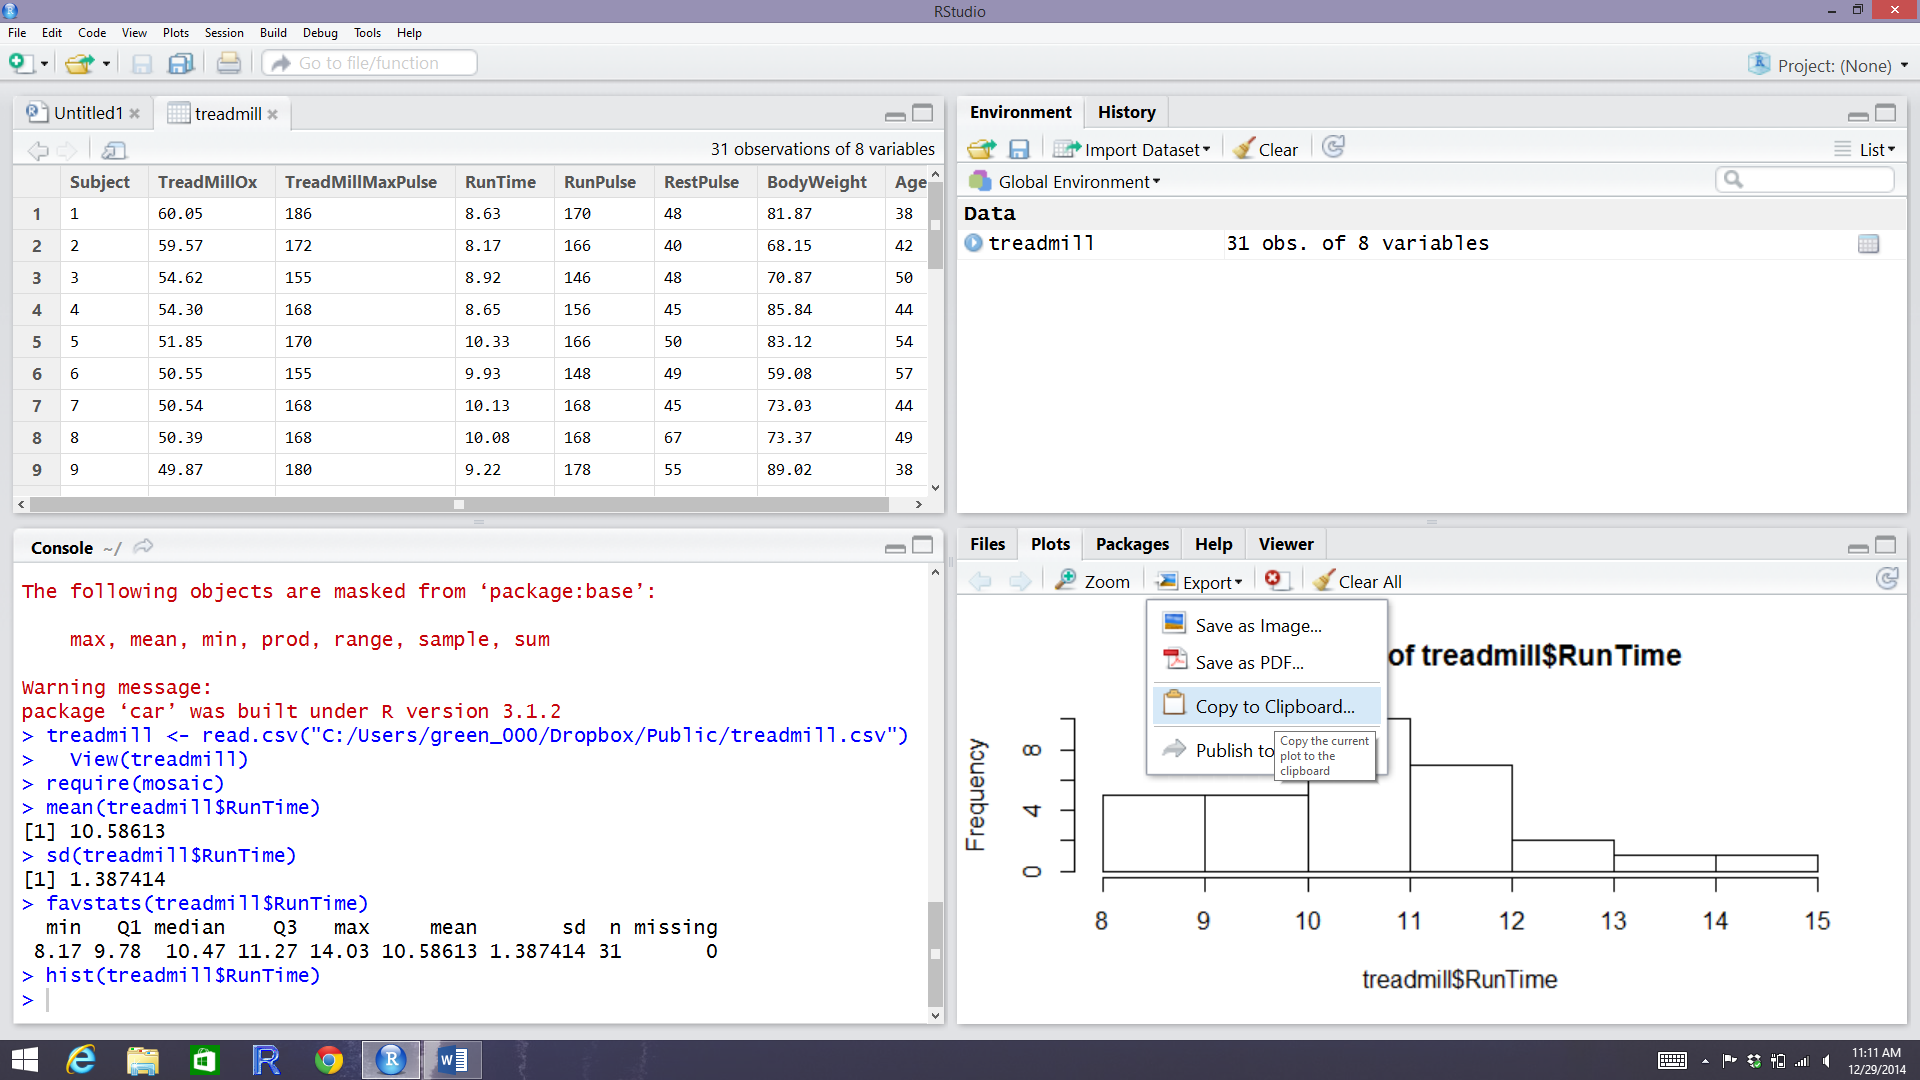
\includegraphics[width=26.67in]{chapter1_files/image010} \caption{RStudio while in the process of copying the histogram.}\label{fig:Figure1-6}
\end{figure}

\indent The function \texttt{hist} defaults into providing a histogram on the \textbf{\emph{frequency}}
(count) scale. In most R functions, there are the default options that will
occur if we don't make any specific choices but we
can override the default options if we desire. One option we can modify here is
to add labels to the bars to be able to see exactly how many observations fell
into each bar. Specifically, we can turn the \texttt{labels} option ``on'' by making it true (``T'') by adding \texttt{labels=T} to the previous call to the \texttt{hist} function, separated by a comma. Note that we will use the \texttt{=} sign only for changing options within functions.

\begin{Shaded}
\begin{Highlighting}[]
\OperatorTok{>}\StringTok{ }\KeywordTok{hist}\NormalTok{(treadmill}\OperatorTok{$}\NormalTok{RunTime, }\DataTypeTok{labels=}\NormalTok{T)}
\end{Highlighting}
\end{Shaded}



\begin{figure}
\centering
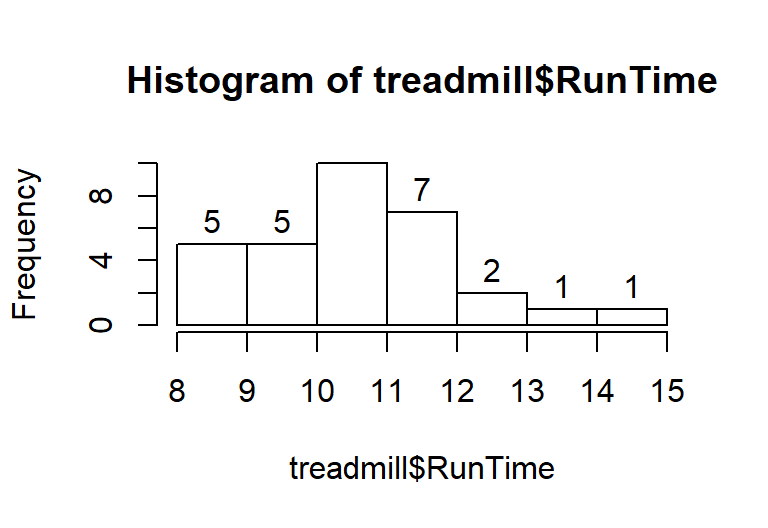
\includegraphics{01-preface_files/figure-latex/Figure1-7-1.pdf}
\caption{\label{fig:Figure1-7}Histogram of Run Times with counts in bars labeled.}
\end{figure}

\indent Based on this histogram, it does not appear that there any outliers in the responses
since there are no bars that are separated from the other observations. However,
the distribution does not look symmetric and there might be a skew to the
distribution. Specifically, it appears to be \textbf{\emph{skewed right}} (the right tail is longer than the left). But histograms can sometimes mask features of
the data set by binning observations and it is hard to find the percentiles
accurately from the plot.

\indent When assessing outliers and skew, the \textbf{\emph{boxplot}}
(or \emph{Box and Whiskers} plot) can also be helpful (Figure \ref{fig:Figure1-8}) to describe the
shape of the distribution as it displays the 5-number summary and will also indicate
observations that are ``far'' above the middle of the observations.
\index{boxplot}
R's \texttt{boxplot} function uses the standard rule to indicate an observation as a
\textbf{\emph{potential outlier}} if it falls more than 1.5 times the \textbf{\emph{IQR}}
(Inter-Quartile Range, calculated as Q3 -- Q1) below Q1 or above Q3.
\index{outlier}
The potential outliers
are plotted with circles and the \emph{Whiskers} (lines that extend from Q1 and Q3 typically to
the minimum and maximum) are shortened to only go as far as
observations that are within \(1.5*\)IQR of the upper and lower quartiles. The \emph{box}
part of the boxplot is a box that goes from Q1 to Q3 and the median is displayed as a line
somewhere inside the box.\footnote{The median, quartiles and whiskers sometimes occur at the same
  values when there are many tied observations. If you can't see all the
  components of the boxplot, produce the numerical summary to help you understand
  what happened.} Looking back at the summary statistics above, Q1=9.78 and Q3=11.27, providing an IQR of:

\begin{Shaded}
\begin{Highlighting}[]
\OperatorTok{>}\StringTok{ }\NormalTok{IQR <-}\StringTok{ }\FloatTok{11.27} \OperatorTok{-}\StringTok{ }\FloatTok{9.78}
\OperatorTok{>}\StringTok{ }\NormalTok{IQR}
\NormalTok{[}\DecValTok{1}\NormalTok{] }\FloatTok{1.49}
\end{Highlighting}
\end{Shaded}

One observation (the maximum value of 14.03) is indicated as a potential outlier
based on this result by being larger than Q3 \(+1.5*\)IQR, which was 13.505:

\begin{Shaded}
\begin{Highlighting}[]
\OperatorTok{>}\StringTok{ }\FloatTok{11.27} \OperatorTok{+}\StringTok{ }\FloatTok{1.5}\OperatorTok{*}\NormalTok{IQR}
\NormalTok{[}\DecValTok{1}\NormalTok{] }\FloatTok{13.505}
\end{Highlighting}
\end{Shaded}

\indent The boxplot also shows a slight indication of a right skew (skew towards
larger values) with the distance from the minimum to the median being smaller than the
distance from the median to the maximum. Additionally, the distance from Q1 to
the median is smaller than the distance from the median to Q3. It is modest skew,
but worth noting.



\begin{figure}
\centering
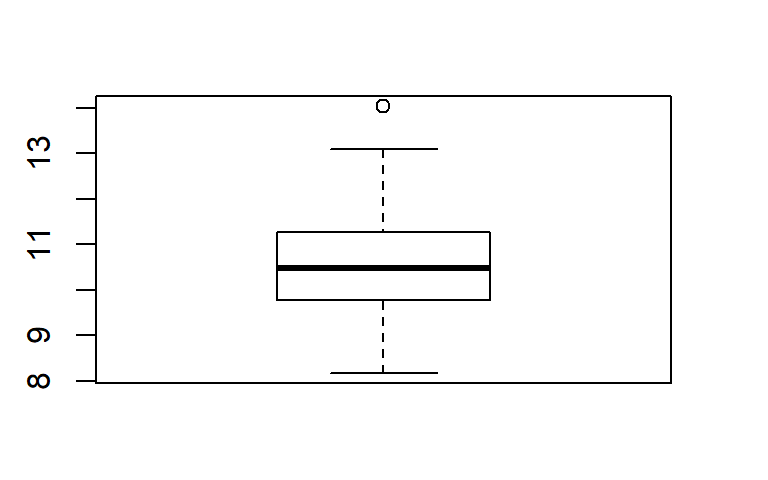
\includegraphics{01-preface_files/figure-latex/Figure1-8-1.pdf}
\caption{\label{fig:Figure1-8}Boxplot of 1.5 mile Run Times.}
\end{figure}

\begin{Shaded}
\begin{Highlighting}[]
\OperatorTok{>}\StringTok{ }\KeywordTok{boxplot}\NormalTok{(treadmill}\OperatorTok{$}\NormalTok{RunTime)}
\end{Highlighting}
\end{Shaded}

\indent While the default boxplot is fine, it fails to provide good graphical labels,
especially on the y-axis. Additionally, there is no title on the plot. The
following code provides some enhancements to the plot by using the \texttt{ylab} and
\texttt{main} options in the call to \texttt{boxplot}, with the results displayed in
Figure \ref{fig:Figure1-9}. When we add text to plots, it will be contained within quotes and
be assigned into the options \texttt{ylab} (for y-axis) or \texttt{main}
(for the title) here to put it into those locations.



\begin{figure}
\centering
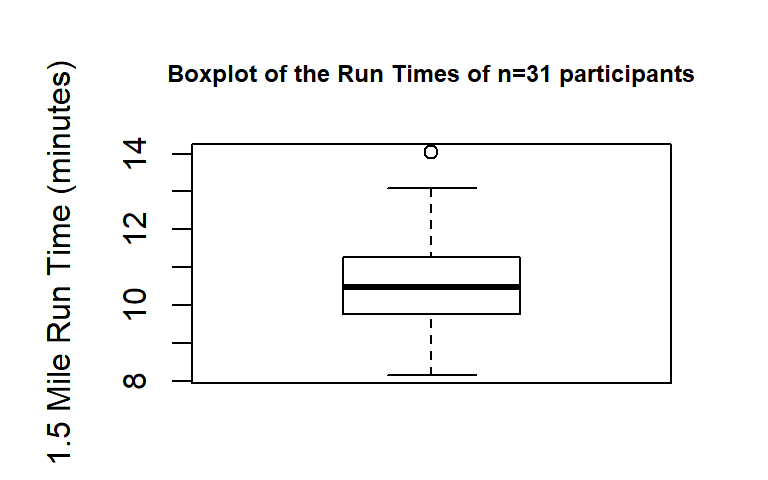
\includegraphics{01-preface_files/figure-latex/Figure1-9-1.pdf}
\caption{\label{fig:Figure1-9}Boxplot of Run Times with improved labels.}
\end{figure}

\begin{Shaded}
\begin{Highlighting}[]
\OperatorTok{>}\StringTok{ }\KeywordTok{boxplot}\NormalTok{(treadmill}\OperatorTok{$}\NormalTok{RunTime, }\DataTypeTok{ylab=}\StringTok{"1.5 Mile Run Time (minutes)"}\NormalTok{, }
          \DataTypeTok{main=}\StringTok{"Boxplot of the Run Times of n=31 participants"}\NormalTok{)}
\end{Highlighting}
\end{Shaded}

\indent Throughout the book, we will often use extra options to make figures that
are easier for you to understand. There
are often simpler versions of the functions that will suffice but the extra
work to get better labeled figures is often worth it. I guess the point is that
``a picture is worth a thousand words'' but in data visualization, that is only
true if the reader can understand what is being displayed. It is also important
to think about the quality of the information that is being displayed,
regardless of how pretty the graphic might be. So maybe it is better to say
``a picture can be worth a thousand words'' if it is well-labeled?

\indent All the previous results were created by running the R code and then copying the
results from either the console or by copying the figure and then pasting the results
into the typesetting program. There is another way
to use RStudio where you can have it compile the results (both output and
figures) directly into a document together with the code that generated it,
using what is called R Markdown (\url{http://shiny.rstudio.com/articles/rmarkdown.html}).
It adds some additional setup
complexity we want to avoid for now but is basically what we used to prepare this book.
The main reason to mention this is that you will see a
change in formatting of the R code and output from here forward as you will no
longer see the command prompt (``\textgreater{}'') with the code. The output will be
flagged by having two ``\#\#'''s before it. For example, the summary statistics for
the \emph{RunTime} variable from \texttt{favstats} function would look like:

\begin{Shaded}
\begin{Highlighting}[]
\KeywordTok{favstats}\NormalTok{(treadmill}\OperatorTok{$}\NormalTok{RunTime)}
\end{Highlighting}
\end{Shaded}

\begin{verbatim}
##   min   Q1 median    Q3   max     mean       sd  n missing
##  8.17 9.78  10.47 11.27 14.03 10.58613 1.387414 31       0
\end{verbatim}

\indent Statisticians (and other scientists) are starting to use these methods
because they provide what is called ``Reproducible
research'' \citep{Gandrud2015} where all the code and output it produced are
available in a single place. This allows different researchers to run and verify
results or the original researchers to revisit their earlier work at a later
date and recreate all their results exactly. Scientific publications are currently
encouraging researchers to work in this way and may someday require it. In this
book, we focus on the R code and show the results from running it, but you may
want to consider exploring these alternative options. Ask your instructor to show
you this way of working and see if you like it better than copying and pasting everything.

\indent Finally, when you are done with your work and attempt to exit out of RStudio,
it will
ask you to save your workspace. \textbf{\emph{DO NOT DO THIS!}} It will just create a cluttered
workspace and could even cause you to get incorrect results. If you
save your R code (and edit it to only contain the parts of it that worked) via the
script window, you can re-create any results by simply
re-running that code. If you find that you have lots of ``stuff'' in your
workspace because you accidentally saved your workspace, just run \texttt{rm(list\ =\ ls())}.
It will delete all the data sets from your workspace.

\hypertarget{section1-4}{%
\section{Chapter summary}\label{section1-4}}

This chapter covered getting R and RStudio downloaded and some basics of working with
R via RStudio. You should be able to read a data set into R and run some basic
functions, all done using the RStudio interface. If you are struggling with
this, you should seek additional help with these technical issues so that you
are ready for more complicated statistical methods that are going to be
encountered in the following chapters. For most assignments, we will give you a
seed of the basic R code that you need and then you will modify it to work on
your data set of interest. As mentioned previously, the way everyone learns R is
by starting with some example code that does most of what you want to do and
then you modify it. If you can complete the Practice Problems that follow, you
are well on your way to learning to use R.

\indent The statistical methods in this chapter were minimal and all should have been
review. They involved a quick reminder of summarizing the center, spread, and
shape of distributions using numerical summaries of the mean and SD and/or the
min, Q1, median, Q3, and max and the histogram and boxplot as graphical
summaries. We revisited the ideas of symmetry and skew. But the main point was
really to get a start on using R to provide results you should be familiar with
from your previous statistics experience(s).

\hypertarget{section1-5}{%
\section{Summary of important R code}\label{section1-5}}

To help you learn and use R, there is a section highlighting the most important
R code used near the end of each
chapter. The bold text will never change but the
lighter and/or ALL CAPS text (red in the online or digital version) will need
to be customized to your particular application. The sub-bullet for each
function will discuss the use of the function and pertinent options or packages
required. You can use this as a guide to finding the function names and some
hints about options that will help you to get the code to work. You can also
revisit the worked examples using each of the functions.

\begin{itemize}
\item
  \textcolor{red}{FILENAME} \texttt{\textless{}-} \textbf{read\_csv(}\textcolor{red}{"path to csv file/FILENAME.csv"}\textbf{)}

  \begin{itemize}
  \item
    Can be generated using ``Import Dataset'' button or by modifying this text.
  \item
    Requires the \texttt{readr} package to be loaded (\texttt{require(readr)}) when using
    the code directly.
  \item
    Imports a text file saved in the CSV format.
  \end{itemize}
\item
  \textcolor{red}{DATASETNAME}\textbf{\$}\textcolor{red}{VARIABLENAME}

  \begin{itemize}
  \tightlist
  \item
    To access a particular variable in a tibble called DATASETNAME, use
    a \$ and then the VARIABLENAME.
  \end{itemize}
\item
  \textbf{head(}\textcolor{red}{DATASETNAME}\textbf{)}

  \begin{itemize}
  \tightlist
  \item
    Provides a list of the first few rows of the data set for all the
    variables in it. \index{\texttt{head()}|textbf}
  \end{itemize}
\item
  \textbf{tail(}\textcolor{red}{DATASETNAME}\textbf{)}

  \begin{itemize}
  \tightlist
  \item
    Provides a list of the last few rows of the data set for all the
    variables in it. \index{\texttt{tail()}|textbf}
  \end{itemize}
\item
  \textbf{mean(}\textcolor{red}{DATASETNAME}\textbf{\$}\textcolor{red}{VARIABLENAME}\textbf{)}

  \begin{itemize}
  \tightlist
  \item
    Calculates the mean of the observations in a variable.
    \index{\texttt{mean()}|textbf}
  \end{itemize}
\item
  \textbf{sd(}\textcolor{red}{DATASETNAME}\textbf{\$}\textcolor{red}{VARIABLENAME}\textbf{)}

  \begin{itemize}
  \tightlist
  \item
    Calculates the standard deviation of the observations in a variable.
    \index{\texttt{sd()}|textbf}
  \end{itemize}
\item
  \textbf{favstats(}\textcolor{red}{DATASETNAME}\$\textcolor{red}{VARIABLENAME}\textbf{)}

  \begin{itemize}
  \item
    Requires the \texttt{mosaic} package to be loaded (\texttt{require(mosaic}) after
    installing the package).
  \item
    Provides a suite of numerical summaries of the observations in a variable.
    \index{\texttt{favstats()}|textbf}
  \end{itemize}
\item
  \textbf{hist(}\textcolor{red}{DATASETNAME}\textbf{\$}\textcolor{red}{VARIABLENAME}\textbf{)}

  \begin{itemize}
  \tightlist
  \item
    Makes a histogram. \index{\texttt{hist()}|textbf}
  \end{itemize}
\item
  \textbf{boxplot(}\textcolor{red}{DATASETNAME}\textbf{\$}\textcolor{red}{VARIABLENAME}\textbf{)}

  \begin{itemize}
  \tightlist
  \item
    Makes a boxplot. \index{\texttt{boxplot()}|textbf}
  \end{itemize}
\end{itemize}

\hypertarget{section1-6}{%
\section{Practice problems}\label{section1-6}}

In each chapter, the last section contains some questions for you to complete
to make sure you understood the
material. You can download the code to answer questions 1.1 to 1.5 below at
\url{http://www.math.montana.edu/courses/s217/documents/Ch1.Rmd}. But to practice
learning R, it would be most useful for you to try to accomplish the requested tasks
yourself and then only refer to the provided R code if/when you struggle.
These questions provide a great venue to check your learning, often to see the
methods applied to another data set, and for something to discuss in study groups,
with your instructor, and at the Math Learning Center.

1.1. Read in the treadmill data set
discussed previously and find the mean and SD of the Ages (\texttt{Age} variable) and Body
Weights (\texttt{BodyWeight} variable). In studies involving human subjects, it is
common to report a
summary of characteristics of the subjects. Why does this matter? Think about
how your interpretation of any study of the fitness of subjects would change if
the mean age (same spread) had been 20 years older or 35 years younger.

1.2. How does knowing about the
distribution of results for \emph{Age} and \emph{BodyWeight} help you understand the
results for the Run Times discussed previously?

1.3. The mean and SD are most useful
as summary statistics only if the distribution is relatively symmetric. Make a
histogram of \emph{Age} responses and
discuss the shape of the distribution (is it skewed right, skewed left,
approximately symmetric?; are there outliers?). Approximately what range of
ages does this study pertain to?

1.4. The weight responses are in
kilograms and you might prefer to see them in pounds. The conversion is
lbs=2.205\texttt{*}kgs. Create a new variable in the \texttt{treadmill}
tibble called \emph{BWlb} using this code:

\begin{Shaded}
\begin{Highlighting}[]
\NormalTok{treadmill}\OperatorTok{$}\NormalTok{BWlb <-}\StringTok{ }\FloatTok{2.205}\OperatorTok{*}\NormalTok{treadmill}\OperatorTok{$}\NormalTok{BodyWeight}
\end{Highlighting}
\end{Shaded}

and find the mean and SD of the new variable (\emph{BWlb}).

1.5. Make histograms and boxplots of
the original \emph{BodyWeight} and new \emph{BWlb} variables. Discuss aspects of the
distributions that changed and those that remained the same with the
transformation from kilograms to pounds. What does this tell you about changing the units of a variable in terms of its distribution?

\hypertarget{chapter2}{%
\chapter{(R)e-Introduction to statistics}\label{chapter2}}

Placeholder

\hypertarget{section2-3}{%
\section{Models, hypotheses, and permutations for the two sample mean situation}\label{section2-3}}

\hypertarget{section2-4}{%
\section{Permutation testing for the two sample mean situation}\label{section2-4}}

\hypertarget{section2-5}{%
\section{Hypothesis testing (general)}\label{section2-5}}

\hypertarget{section2-6}{%
\section{Connecting randomization (nonparametric) and parametric tests}\label{section2-6}}

\hypertarget{section2-7}{%
\section{Second example of permutation tests}\label{section2-7}}

\hypertarget{section2-8}{%
\section{Confidence intervals and bootstrapping}\label{section2-8}}

\hypertarget{section2-9}{%
\section{Bootstrap confidence intervals for difference in GPAs}\label{section2-9}}

\hypertarget{section2-10}{%
\section{Chapter summary}\label{section2-10}}

\hypertarget{section2-11}{%
\section{Summary of important R code}\label{section2-11}}

\hypertarget{section2-12}{%
\section{Practice problems}\label{section2-12}}

\hypertarget{chapter3}{%
\chapter{One-Way ANOVA}\label{chapter3}}

Placeholder

\hypertarget{section3-1}{%
\section{Situation}\label{section3-1}}

\hypertarget{section3-2}{%
\section{Linear model for One-Way ANOVA (cell-means and reference-coding)}\label{section3-2}}

\hypertarget{section3-3}{%
\section{One-Way ANOVA Sums of Squares, Mean Squares, and F-test}\label{section3-3}}

\hypertarget{section3-4}{%
\section{ANOVA model diagnostics including QQ-plots}\label{section3-4}}

\hypertarget{section3-5}{%
\section{Guinea pig tooth growth One-Way ANOVA example}\label{section3-5}}

\hypertarget{section3-6}{%
\section{Multiple (pair-wise) comparisons using Tukey's HSD and the compact letter display}\label{section3-6}}

\hypertarget{section3-7}{%
\section{Pair-wise comparisons for Prisoner Rating data}\label{section3-7}}

\hypertarget{section3-8}{%
\section{Chapter summary}\label{section3-8}}

\hypertarget{section3-9}{%
\section{Summary of important R code}\label{section3-9}}

\hypertarget{section3-10}{%
\section{Practice problems}\label{section3-10}}

\hypertarget{chapter4}{%
\chapter{Two-Way ANOVA}\label{chapter4}}

Placeholder

\hypertarget{section4-1}{%
\section{Situation}\label{section4-1}}

\hypertarget{section4-2}{%
\section{Designing a two-way experiment and visualizing results}\label{section4-2}}

\hypertarget{section4-3}{%
\section{Two-Way ANOVA models and hypothesis tests}\label{section4-3}}

\hypertarget{section4-4}{%
\section{Guinea pig tooth growth analysis with Two-Way ANOVA}\label{section4-4}}

\hypertarget{section4-5}{%
\section{Observational study example: The Psychology of Debt}\label{section4-5}}

\hypertarget{section4-6}{%
\section{Pushing Two-Way ANOVA to the limit: Un-replicated designs}\label{section4-6}}

\hypertarget{section4-7}{%
\section{Chapter summary}\label{section4-7}}

\hypertarget{section4-8}{%
\section{Summary of important R code}\label{section4-8}}

\hypertarget{section4-9}{%
\section{Practice problems}\label{section4-9}}

\hypertarget{chapter5}{%
\chapter{Chi-square tests}\label{chapter5}}

Placeholder

\hypertarget{section5-1}{%
\section{Situation, contingency tables, and tableplots}\label{section5-1}}

\hypertarget{section5-2}{%
\section{Homogeneity test hypotheses}\label{section5-2}}

\hypertarget{section5-3}{%
\section{Independence test hypotheses}\label{section5-3}}

\hypertarget{section5-4}{%
\section{Models for R by C tables}\label{section5-4}}

\hypertarget{section5-5}{%
\section{\texorpdfstring{Permutation tests for the \(X^2\) statistic}{Permutation tests for the X\^{}2 statistic}}\label{section5-5}}

\hypertarget{section5-6}{%
\section{\texorpdfstring{Chi-square distribution for the \(X^2\) statistic}{Chi-square distribution for the X\^{}2 statistic}}\label{section5-6}}

\hypertarget{section5-7}{%
\section{Examining residuals for the source of differences}\label{section5-7}}

\hypertarget{section5-8}{%
\section{\texorpdfstring{General protocol for \(X^2\) tests}{General protocol for X\^{}2 tests}}\label{section5-8}}

\hypertarget{section5-9}{%
\section{Political party and voting results: Complete analysis}\label{section5-9}}

\hypertarget{section5-10}{%
\section{Is cheating and lying related in students?}\label{section5-10}}

\hypertarget{section5-11}{%
\section{Analyzing a stratified random sample of California schools}\label{section5-11}}

\hypertarget{section5-12}{%
\section{Chapter summary}\label{section5-12}}

\hypertarget{section5-13}{%
\section{Summary of important R commands}\label{section5-13}}

\hypertarget{section5-14}{%
\section{Practice problems}\label{section5-14}}

\hypertarget{chapter6}{%
\chapter{Correlation and Simple Linear Regression}\label{chapter6}}

Placeholder

\hypertarget{section6-1}{%
\section{Relationships between two quantitative variables}\label{section6-1}}

\hypertarget{section6-2}{%
\section{Estimating the correlation coefficient}\label{section6-2}}

\hypertarget{section6-3}{%
\section{Relationships between variables by groups}\label{section6-3}}

\hypertarget{section6-4}{%
\section{Inference for the correlation coefficient (Optional section)}\label{section6-4}}

\hypertarget{section6-5}{%
\section{Are tree diameters related to tree heights?}\label{section6-5}}

\hypertarget{section6-6}{%
\section{Describing relationships with a regression model}\label{section6-6}}

\hypertarget{section6-7}{%
\section{Least Squares Estimation}\label{section6-7}}

\hypertarget{section6-8}{%
\section{\texorpdfstring{Measuring the strength of regressions: R\textsuperscript{2}}{Measuring the strength of regressions: R2}}\label{section6-8}}

\hypertarget{section6-9}{%
\section{Outliers: leverage and influence}\label{section6-9}}

\hypertarget{section6-10}{%
\section{Residual diagnostics -- setting the stage for inference}\label{section6-10}}

\hypertarget{section6-11}{%
\section{Old Faithful discharge and waiting times}\label{section6-11}}

\hypertarget{section6-12}{%
\section{Chapter summary}\label{section6-12}}

\hypertarget{section6-13}{%
\section{Summary of important R code}\label{section6-13}}

\hypertarget{section6-14}{%
\section{Practice problems}\label{section6-14}}

\hypertarget{chapter7}{%
\chapter{Simple linear regression inference}\label{chapter7}}

Placeholder

\hypertarget{section7-1}{%
\section{Model}\label{section7-1}}

\hypertarget{section7-2}{%
\section{Confidence interval and hypothesis tests for the slope and intercept}\label{section7-2}}

\hypertarget{section7-3}{%
\section{Bozeman temperature trend}\label{section7-3}}

\hypertarget{section7-4}{%
\section{Randomizing inferences for the slope coefficient}\label{section7-4}}

\hypertarget{section7-5}{%
\section{Transformations part I: Linearizing relationships}\label{section7-5}}

\hypertarget{section7-6}{%
\section{Transformations part II: Impacts on SLR interpretations: log(y), log(x), \& both log(y) \& log(x)}\label{section7-6}}

\hypertarget{section7-7}{%
\section{Confidence interval for the mean and prediction intervals for a new observation}\label{section7-7}}

\hypertarget{section7-8}{%
\section{Chapter summary}\label{section7-8}}

\hypertarget{section7-9}{%
\section{Summary of important R code}\label{section7-9}}

\hypertarget{section7-10}{%
\section{Practice problems}\label{section7-10}}

\hypertarget{chapter8}{%
\chapter{Multiple linear regression}\label{chapter8}}

Placeholder

\hypertarget{section8-1}{%
\section{Going from SLR to MLR}\label{section8-1}}

\hypertarget{section8-2}{%
\section{Validity conditions in MLR}\label{section8-2}}

\hypertarget{section8-3}{%
\section{Interpretation of MLR terms}\label{section8-3}}

\hypertarget{section8-4}{%
\section{Comparing multiple regression models}\label{section8-4}}

\hypertarget{section8-5}{%
\section{General recommendations for MLR interpretations and VIFs}\label{section8-5}}

\hypertarget{section8-6}{%
\section{MLR inference: Parameter inferences using the t-distribution}\label{section8-6}}

\hypertarget{section8-7}{%
\section{Overall F-test in multiple linear regression}\label{section8-7}}

\hypertarget{section8-8}{%
\section{Case study: First year college GPA and SATs}\label{section8-8}}

\hypertarget{section8-9}{%
\section{Different intercepts for different groups: MLR with indicator variables}\label{section8-9}}

\hypertarget{section8-10}{%
\section{Additive MLR with more than two groups: Headache example}\label{section8-10}}

\hypertarget{section8-11}{%
\section{Different slopes and different intercepts}\label{section8-11}}

\hypertarget{section8-12}{%
\section{F-tests for MLR models with quantitative and categorical variables and interactions}\label{section8-12}}

\hypertarget{section8-13}{%
\section{AICs for model selection}\label{section8-13}}

\hypertarget{section8-14}{%
\section{Case study: Forced expiratory volume model selection using AICs}\label{section8-14}}

\hypertarget{section8-15}{%
\section{Chapter summary}\label{section8-15}}

\hypertarget{section8-16}{%
\section{Summary of important R code}\label{section8-16}}

\hypertarget{section8-17}{%
\section{Practice problems}\label{section8-17}}

\hypertarget{chapter9}{%
\chapter{Case studies}\label{chapter9}}

Placeholder

\hypertarget{section9-1}{%
\section{Overview of material covered}\label{section9-1}}

\hypertarget{section9-2}{%
\section{The impact of simulated chronic nitrogen deposition on the biomass and N2-fixation activity of two boreal feather moss--cyanobacteria associations}\label{section9-2}}

\hypertarget{section9-3}{%
\section{Ants learn to rely on more informative attributes during decision-making}\label{section9-3}}

\hypertarget{section9-4}{%
\section{Multi-variate models are essential for understanding vertebrate diversification in deep time}\label{section9-4}}

\hypertarget{section9-5}{%
\section{What do didgeridoos really do about sleepiness?}\label{section9-5}}

\hypertarget{section9-6}{%
\section{General summary}\label{section9-6}}

\hypertarget{references}{%
\chapter*{References}\label{references}}
\addcontentsline{toc}{chapter}{References}

\bibliography{references.bib,packages.bib}

% end of body code
\cleardoublepage
%\addcontentsline{toc}{chapter}{Index}
\printindex{}


\end{document}
